\documentclass[10pt]{beamer}
\usetheme{Malmoe}
\colorlet{beamer@blendedblue}{green!40!black}
\setbeamertemplate{navigation symbols}{}
\newcommand*\oldmacro{}%
\let\oldmacro\insertshorttitle%
\renewcommand*\insertshorttitle{%
\oldmacro\hfill%
\insertframenumber\,/\,\inserttotalframenumber}

\usepackage{caption}
\usepackage{hyperref}
\usepackage[makeroom]{cancel}
\usepackage{ amssymb }
\usepackage{appendixnumberbeamer}
%\usepackage{tikz-feynman}
\usepackage{graphicx}
\begin{document}
\title{Search for Flavor Changing Neutral Currents in Top Quark Decays}
\subtitle{$t \rightarrow q \gamma$}
\author[Barkeloo]{Jason Barkeloo}

\titlegraphic{
\includegraphics[width=4cm]{../ATLAS-Logo-Ref-RGB.png}\hspace*{2.75cm}~%
   
\includegraphics[width=4cm]{../uo_logo_green_on_white_2.jpg}
}

%\frame{\frametitle{}
%\begin{itemize}
%\item
%\end{itemize}
%}


\date{April 25, 2019}
\frame{\titlepage}
\frame{\frametitle{Overview}\tableofcontents[]}%hidesubsections]}
\section{Brief Background}
%\frame{\frametitle{Table of Contents}\tableofcontents[currentsection,hideothersubsections]}
%%%%%%%%%%%%%%%%%%%%%%%%%%%%%%%%%%%%%%%%%%%%%%%%%%%%%%%%%

\subsection{The Top Quark}
%
%\frame{\frametitle{Top Quark Pair Production}
%\begin{itemize}
%\item Leading order processes for top quark production
%	\begin{itemize}
%	\item Quark-antiquark annihilation $\approx 10\%$
%	\item Gluon-gluon fusion $\approx 90\%$
%	\end{itemize}
%\end{itemize}
%\centering
%
%	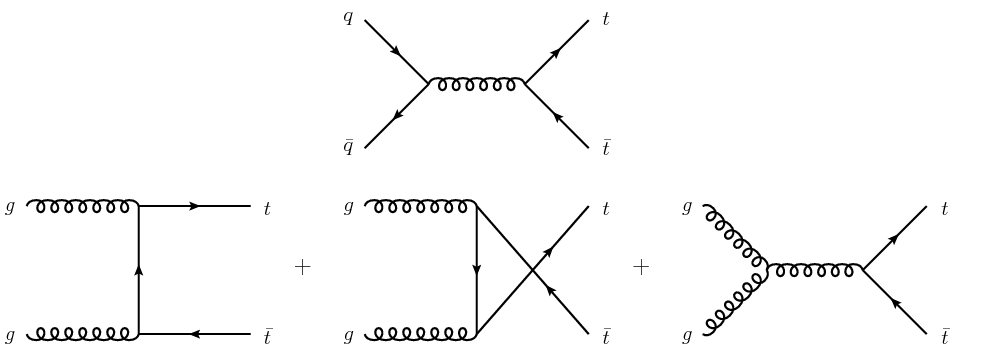
\includegraphics[height=0.4\textheight]{../../Thesis/ThesisImages/LOPairProdDiags.png}
%	\captionof{figure}{Leading order $t\bar{t}$ diagrams}
%}
%
%\frame{\frametitle{Top Quark Pair Production}
%\begin{itemize}
%\item At $\sqrt{s}=13TeV$ for $m_{t}=172.5GeV$, $\sigma_{t\bar{t}} = 831.76pb$
%\end{itemize}
%\centering
%	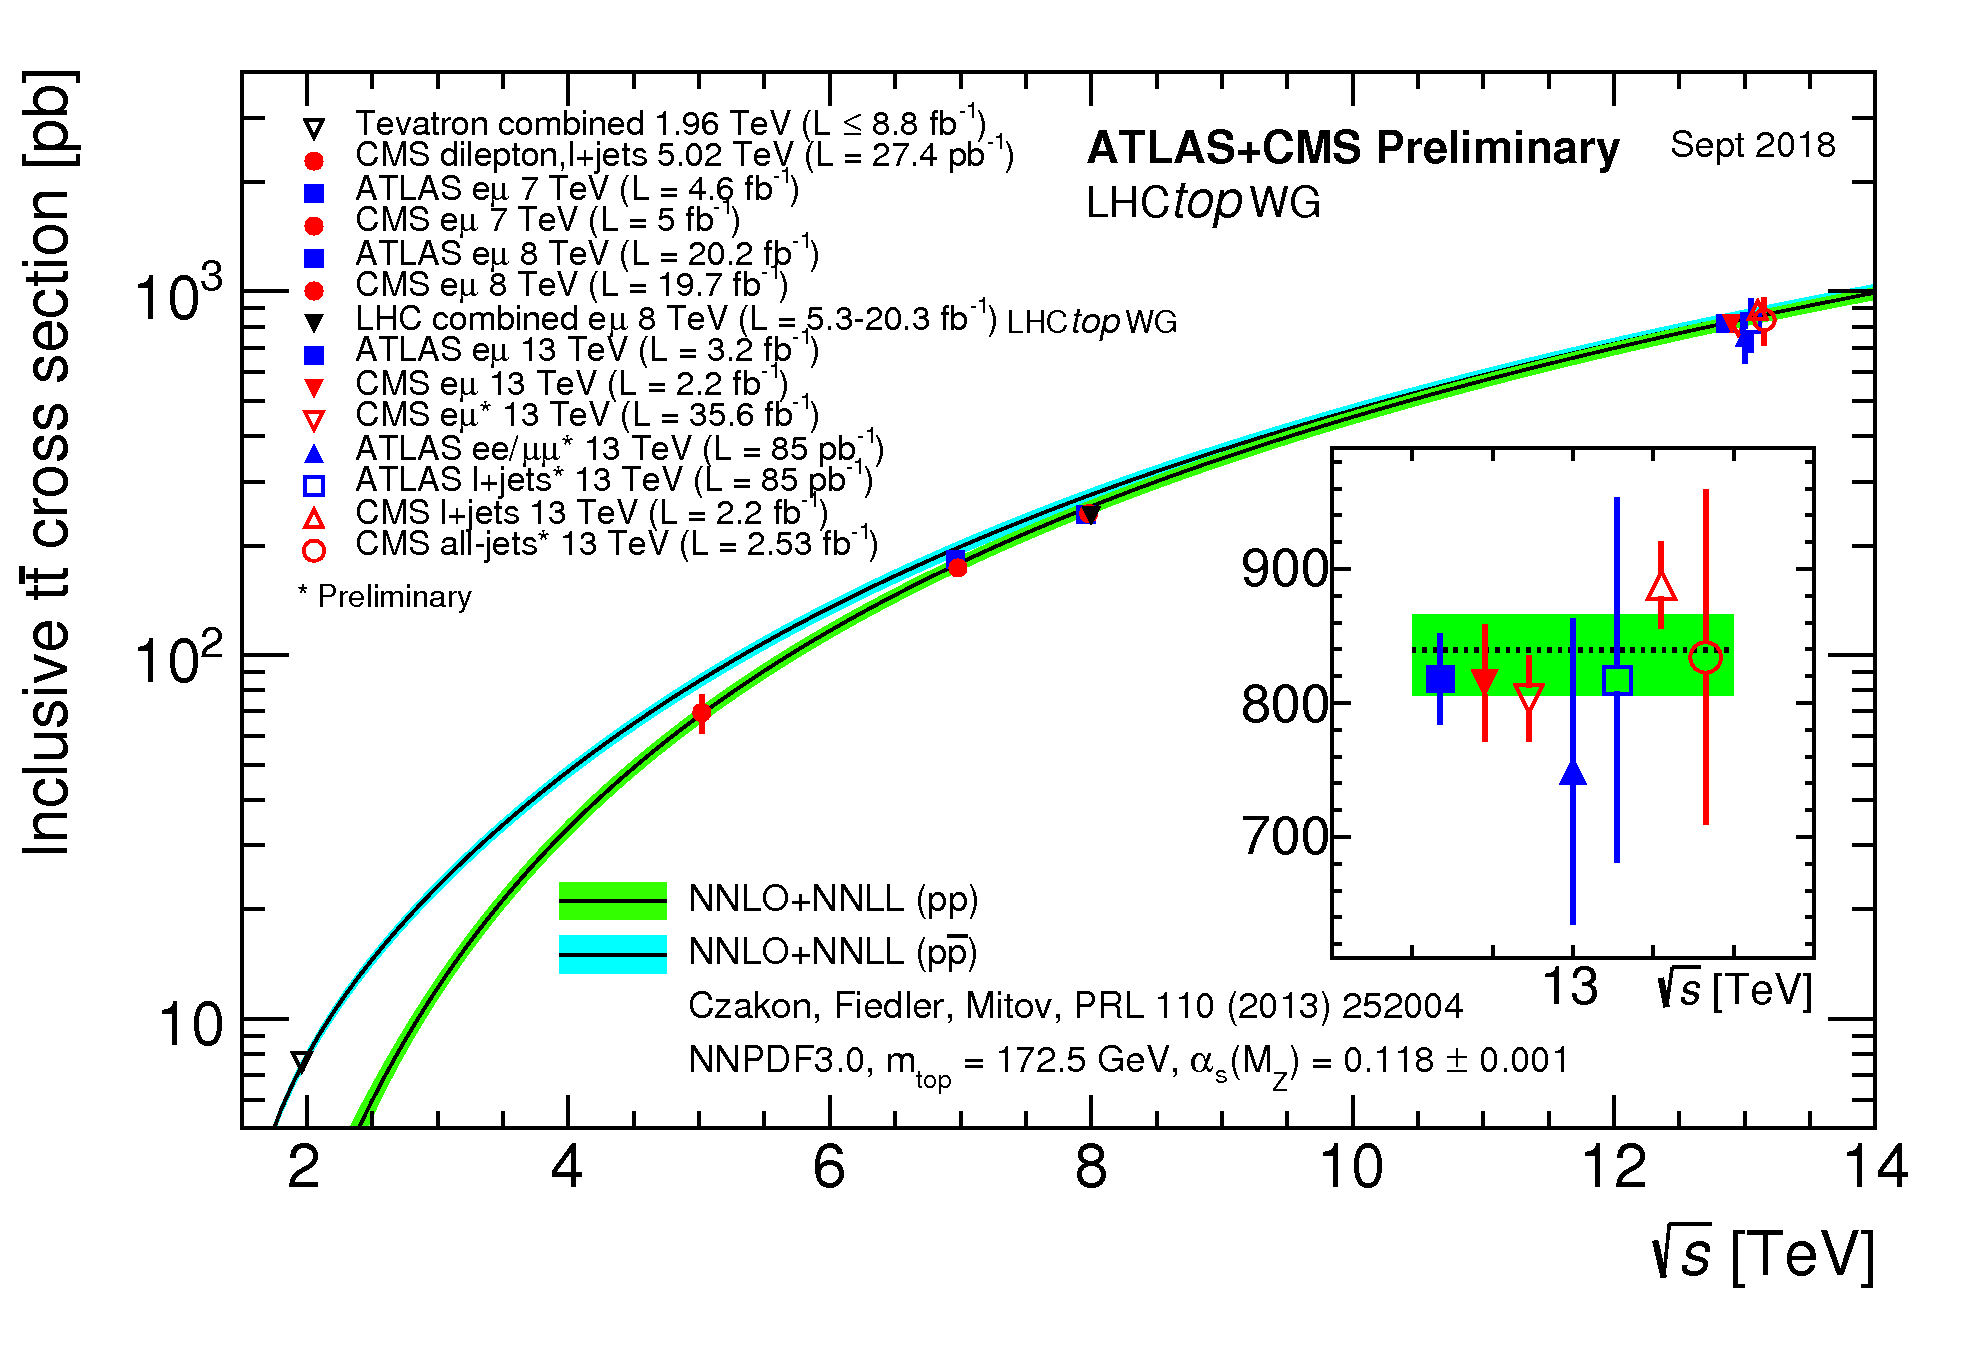
\includegraphics[height=0.7\textheight]{../../Thesis/ThesisImages/ttprodxsec.png}
%	\captionof{figure}{$t\bar{t}$ production cross section \href{https://twiki.cern.ch/twiki/bin/view/LHCPhysics/LHCTopWGSummaryPlots}{[TopWGSummaryPlots]}}
%}
%
%\frame{\frametitle{Top Quark Decays}
%\begin{columns}
%\begin{column}{0.5\textwidth}
%\begin{itemize}
%\item Standard model top branching ratio to bW $\simeq 100\%$
%\end{itemize}
%\centering
% 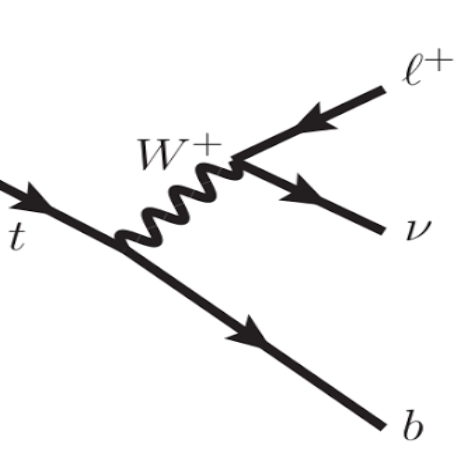
\includegraphics[width=0.7\textwidth]{../../Thesis/ThesisImages/topdecay.png}
% \captionof{figure}{Leptonic final state diagram for a top decay}
%\end{column}
%\begin{column}{0.5\textwidth}  %%<--- here
%     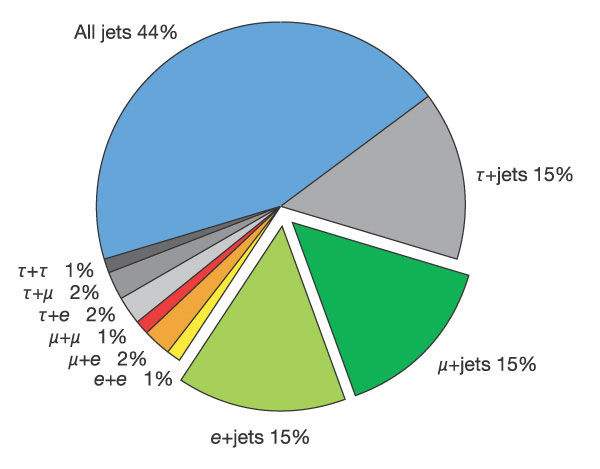
\includegraphics[width=1.1\textwidth]{../../Thesis/ThesisImages/topdecayproducts.jpg}
%    \captionof{figure}{Top quark pair decay final states \href{https://images.nature.com/full/nature-assets/nature/journal/v429/n6992/images/nature02589-f2.2.jpg}{[Nature]}}
%\end{column}
%\end{columns}
%}

\frame{\frametitle{Top Quark Decays in the SM}
\centering
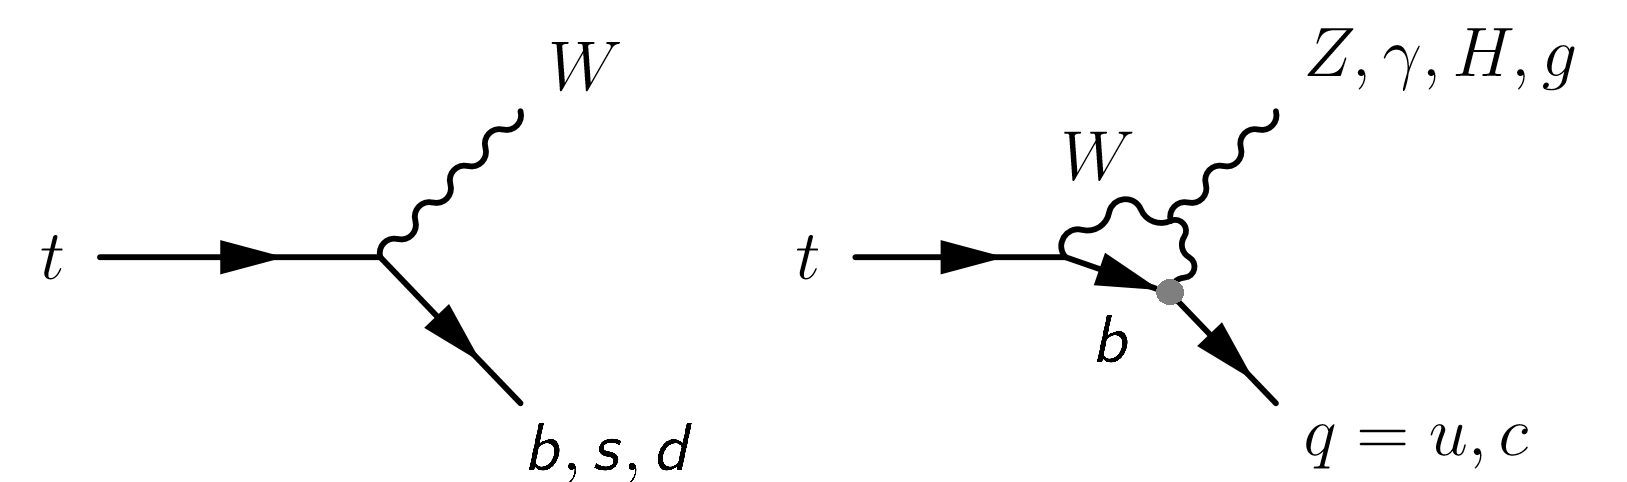
\includegraphics[width=1.\textwidth]{../../Thesis/ThesisImages/SMTopDecays.png}

\begin{columns}
\begin{column}{0.5\textwidth}
\begin{itemize}
\item $t\rightarrow b W \approx 99.83\%$
\item $t\rightarrow s W \approx 0.16\%$
\item $t\rightarrow d W \approx 0.01\%$
\end{itemize}
\end{column}
\begin{column}{0.5\textwidth}
\begin{itemize}
\item $t\rightarrow q_{u,c} X\approx 10^{-17} - 10^{-12}$
\end{itemize}
\end{column}
\end{columns}

%\feynmandiagram [small,horizontal=a to b] {
%  a [particle=\(t\)] -- [fermion] b ,
% f1 [particle=\({b,s,d} \)] -- b -- [boson] f2 [ particle=\(W\)],
%};
}


\frame{\frametitle{Top Flavor Changing Neutral Currents}
\begin{itemize}
\item Current Limits on FCNC Decays
\end{itemize}
\centering
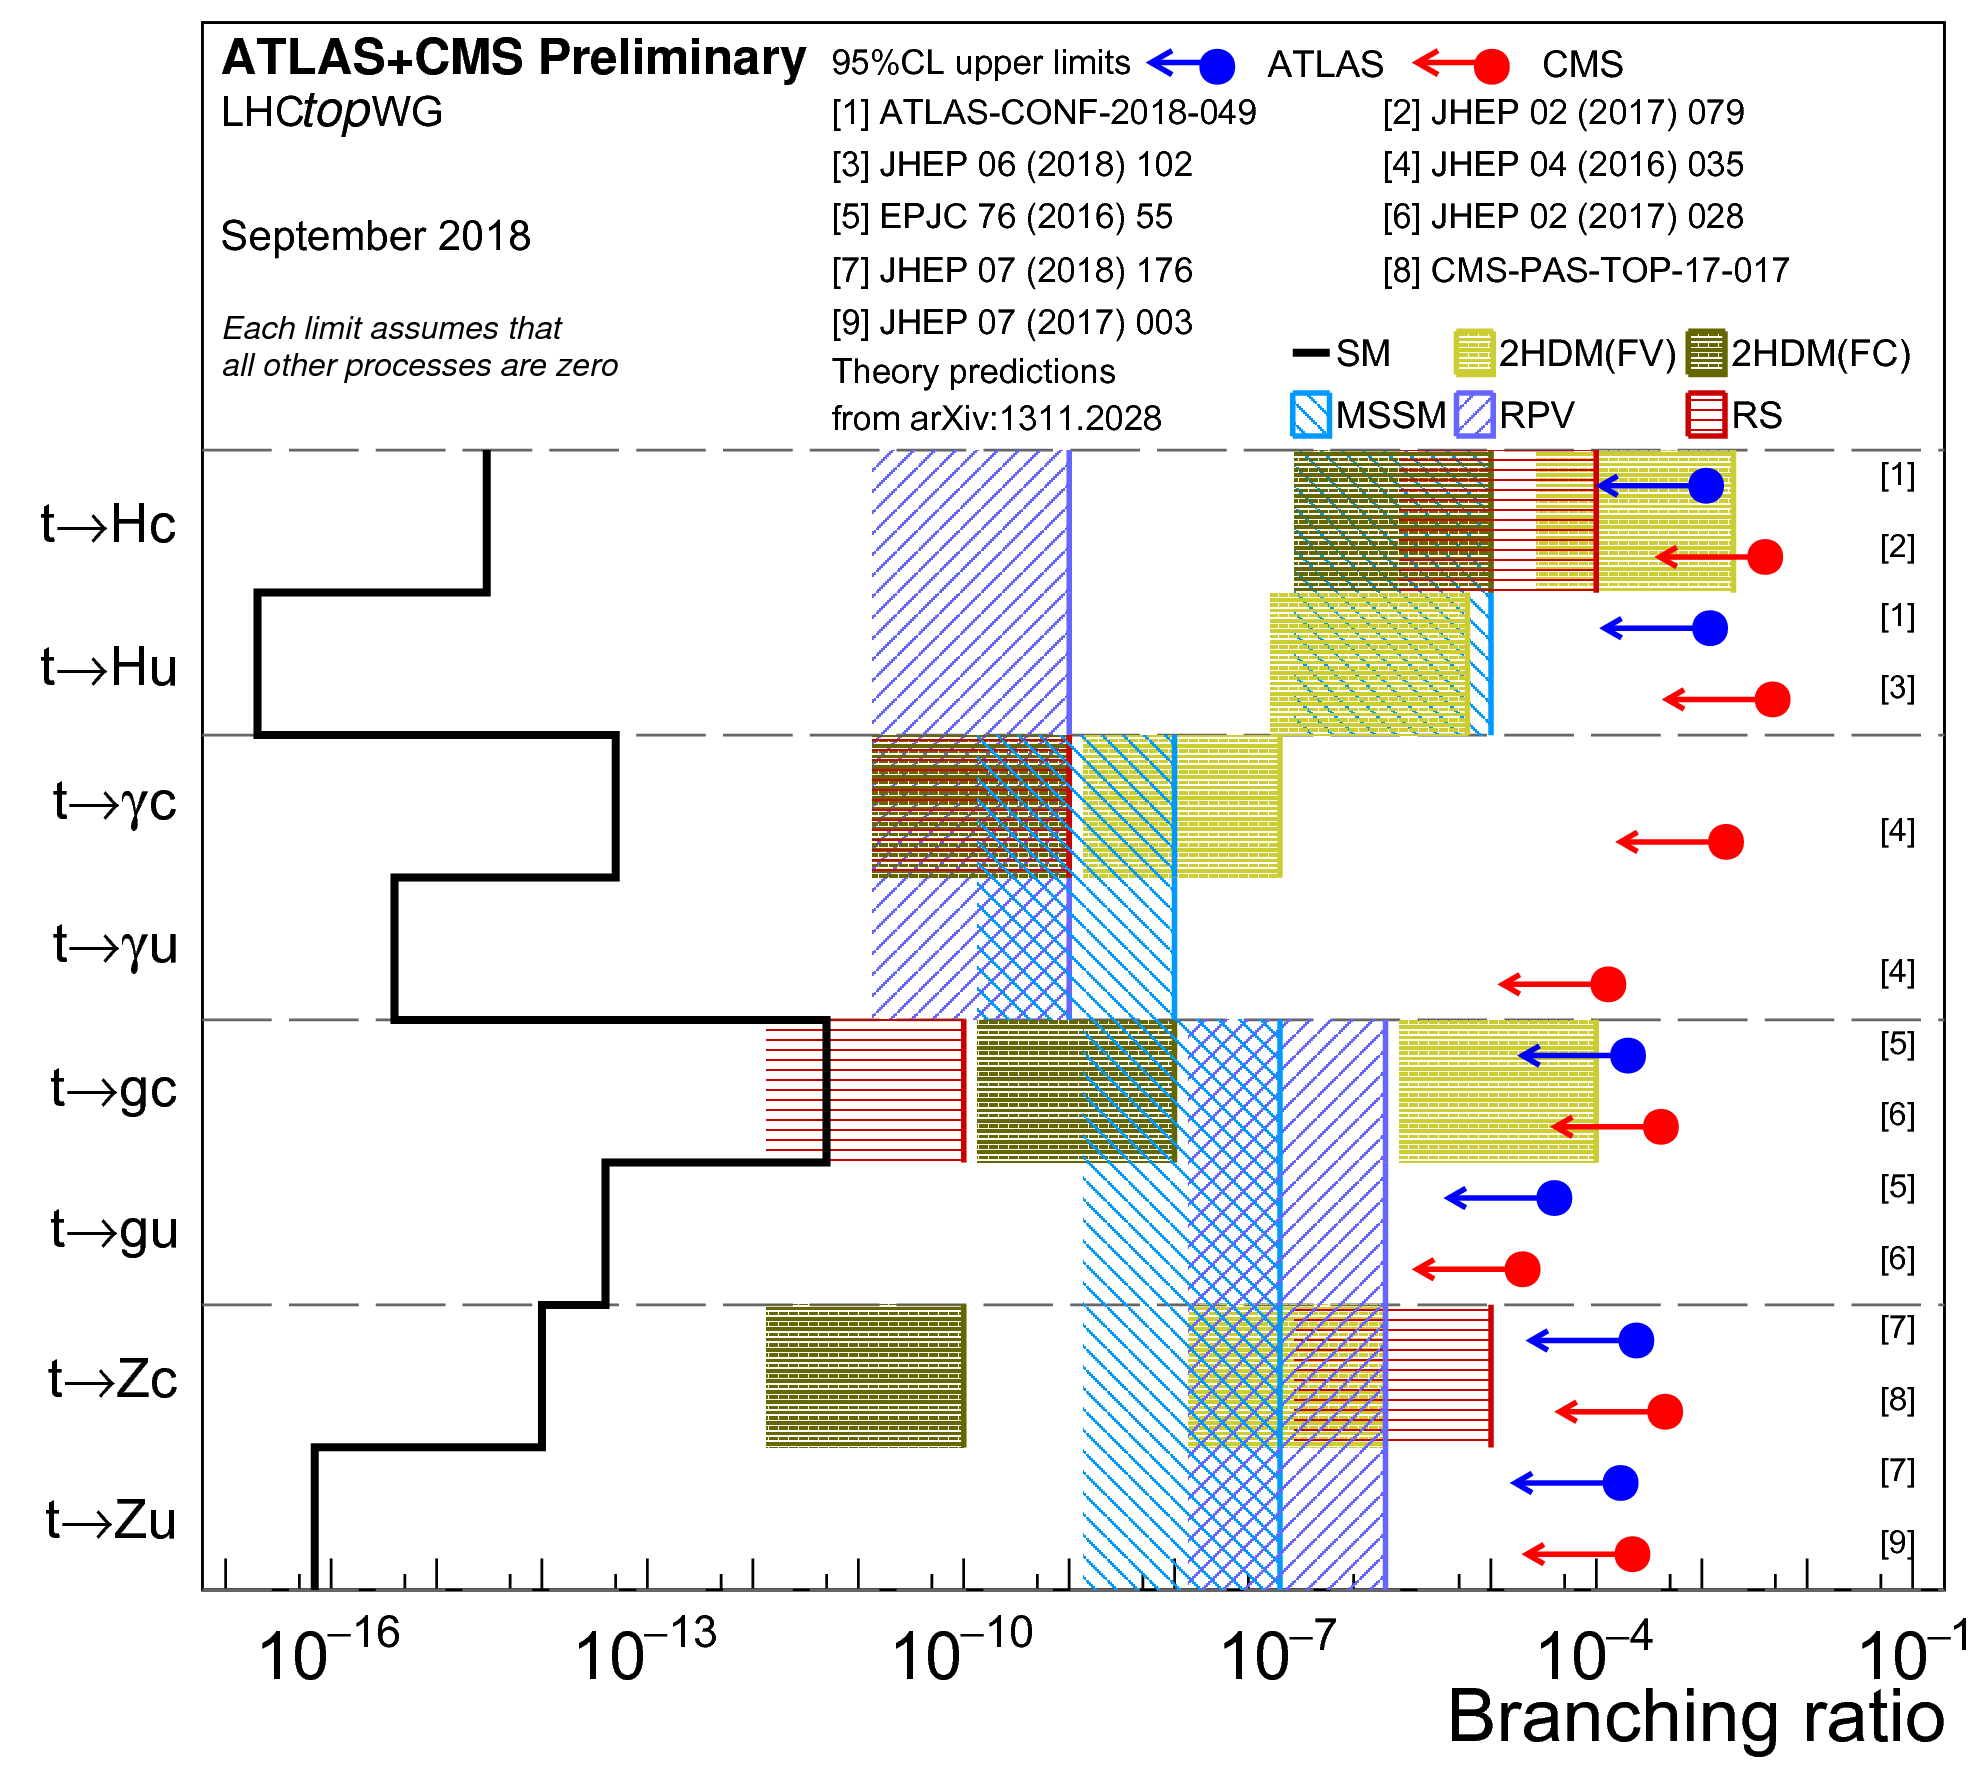
\includegraphics[width=0.55\textwidth]{../../Thesis/ThesisImages/AllFCNCLimits.png}
\begin{itemize}
\item Limits on $t\rightarrow \gamma q$ processes: \href{https://arxiv.org/abs/1511.03951}{[JHEP 04 (2016) 035]}
	\begin{itemize}
	\item $t\rightarrow \gamma u < 1.3 x10^{-4}$
	\item $t\rightarrow \gamma c < 1.7 x 10^{-3}$
	\end{itemize}
\end{itemize}
}

\subsection{FCNC at the LHC} 

\frame{\frametitle{Unpublished Run 1 Limits}
\centering
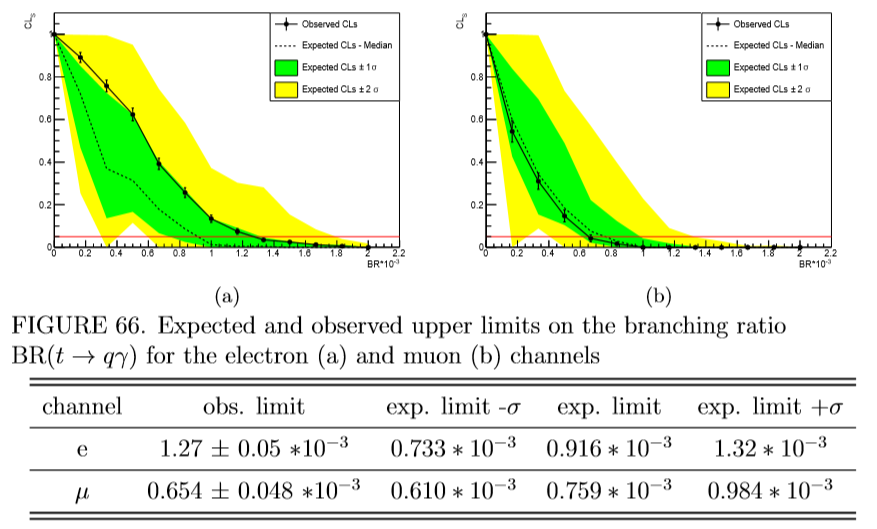
\includegraphics[height=0.6\textheight]{Images/LizaLimit.png}
\begin{itemize}
\item With full Run 2 dataset we expect about 20x more t$\bar{\text{t}}$ pairs, expect significant BR limit improvement in these channels
\item In addition to statistical increase, the use of a neural network should further push down a limit
\end{itemize}
}

\frame{\frametitle{FCNC: What are we looking for? $t\bar{t}\rightarrow W (\rightarrow l \nu) b+ q\gamma$}
\begin{itemize}
\item Final state topology
	\begin{itemize}
	\item One Neutrino, from W
	\item One Lepton, from W
	\item One B-jet, SM Top
	\item One Photon, FCNC Top
	\item One Jet, FCNC Top
	\end{itemize}
\end{itemize}
\centering
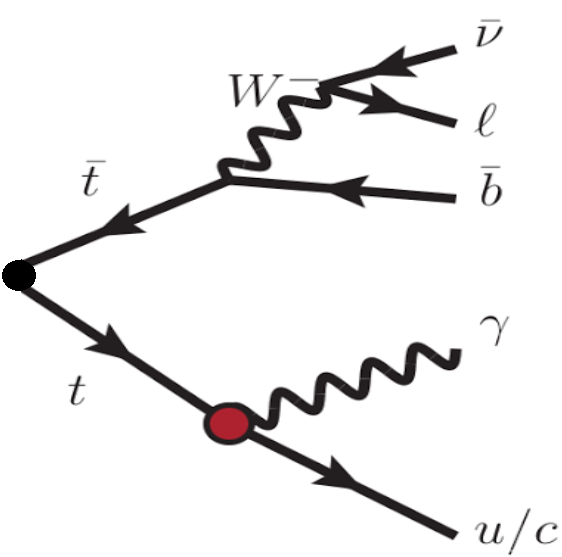
\includegraphics[width=0.4\textwidth]{../../Thesis/ThesisImages/fcncttbar.png}
}

\frame{\frametitle{Background Processes}
\begin{itemize}
\item Due to all of the processes at hadron colliders, it is important to model similar event topologies well
\item Major backgrounds include $t\bar{t}$, W+Jets, Z+Jets, + processes with an associated photon
\end{itemize}
\centering
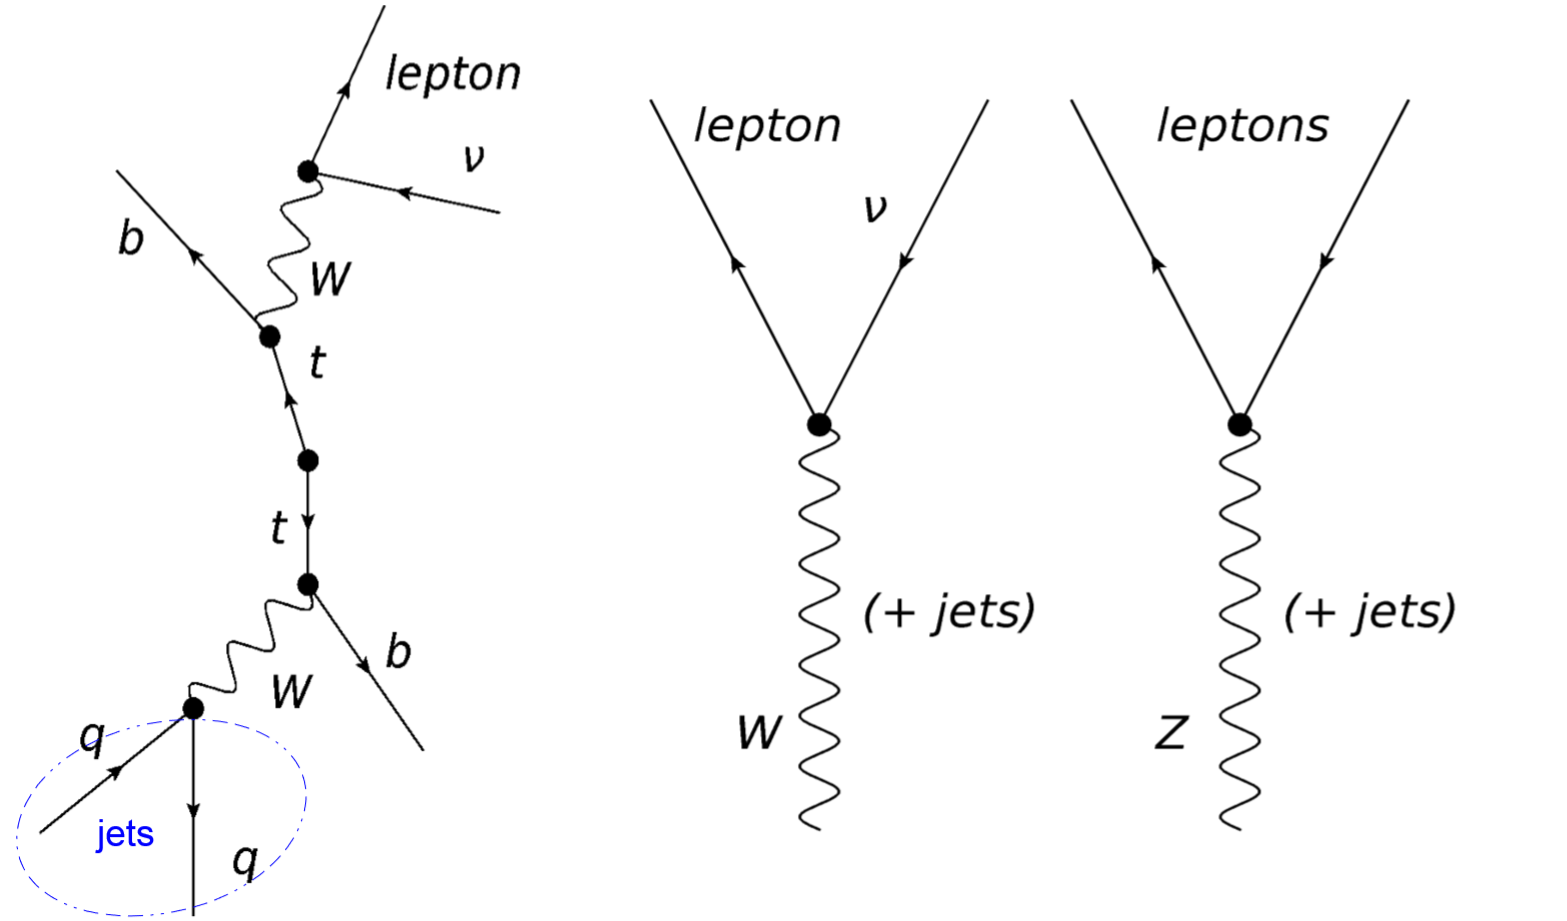
\includegraphics[width=0.7\textwidth]{../../Thesis/ThesisImages/backgrounds.png}
}


\subsection{Transitioning to r21, New Ntuple Production}
\frame{\frametitle{Migration to Release 21}
\begin{itemize}
\item AnalysisTop2.X $\rightarrow$ AnalysisTop21.X
\item Revalidation of UFO Model, Recreation of signal events
\item Custom basic ntuple maker and post-grid local processing code created
\item Parallelization of post-processing code for use with local tier-3 Condor nodes for quicker code testing and analysis
\item Can now do most work off grid in significantly less time
\end{itemize}
}

%%%%%%%%%%%%%%%%%%%%%%%%%%%%%%%%%%%%%%%%%%%%%%%%%%%%%%%%%%%%%%%%%
\section{Searching for Flavor Changing Neutral Current Signatures}

\subsection{FCNCs with Photons}

\subsection{Object Preselection Cuts}


\frame{\frametitle{Object Preselection}
\begin{itemize}
\item We preselect events with objects that look like similar to our expected topology
\item Require:
	\begin{itemize}
	\item Exactly one lepton (e or $\mu$) $\geq$ 28 GeV
	\item Exactly one good photon $\geq$ 15GeV
	\item Missing Transverse Energy $\geq$ 30GeV
	\item $\geq 2$ Jets (at least 1 b-tag)
	\end{itemize}

\end{itemize}
}



\frame{\frametitle{Preselection Objects with $N_{BJet}= 1$ }
\begin{columns}
\begin{column}{0.02\textwidth}
\rotatebox{90}{Muon Channel \qquad  Electron Channel} 
%\rotatebox{90}{Muon Channel        } 
\end{column}
\begin{column}{0.33\textwidth}
\begin{itemize}
\item  Leading Jet $p_T$
\end{itemize}
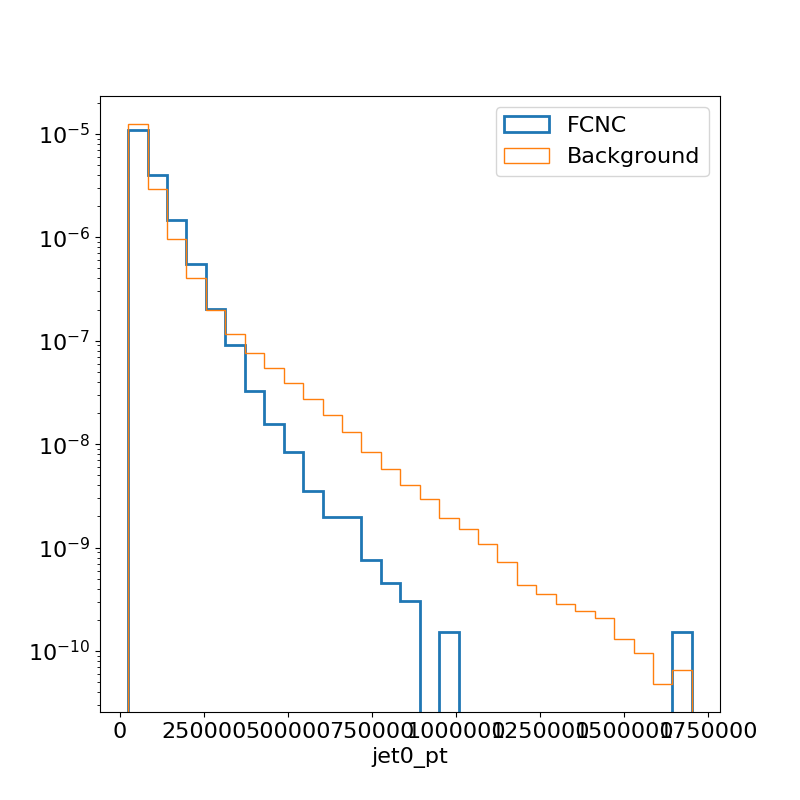
\includegraphics[width=.85\textwidth]{Images/ejetsvarplots/jet0_pt.png} \\
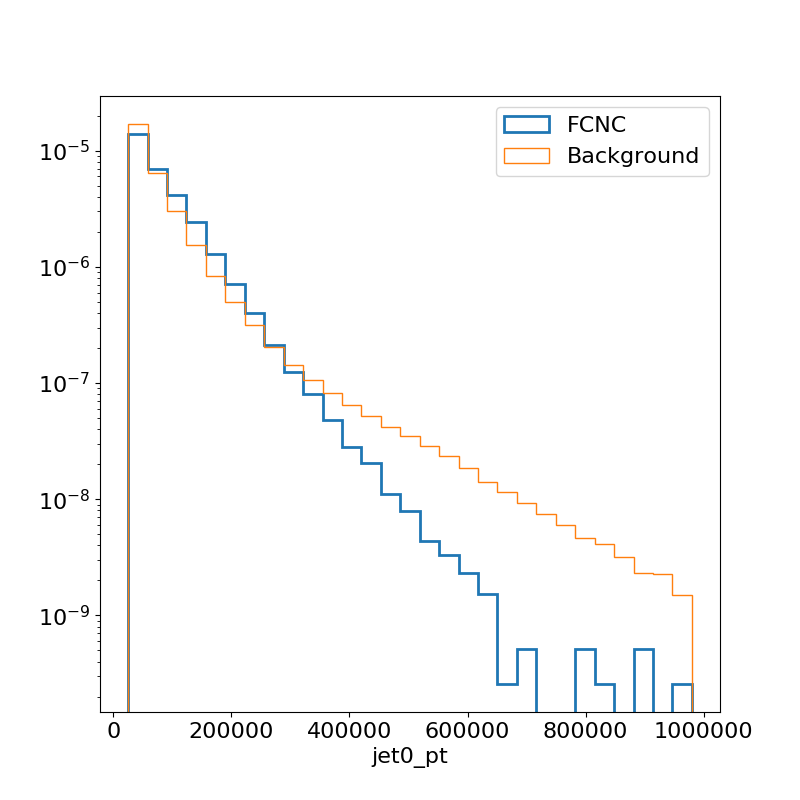
\includegraphics[width=.85\textwidth]{Images/mujetsvarplots/jet0_pt.png}
\end{column}
\begin{column}{0.33\textwidth}
\begin{itemize}
\item Lead Photon
\end{itemize}
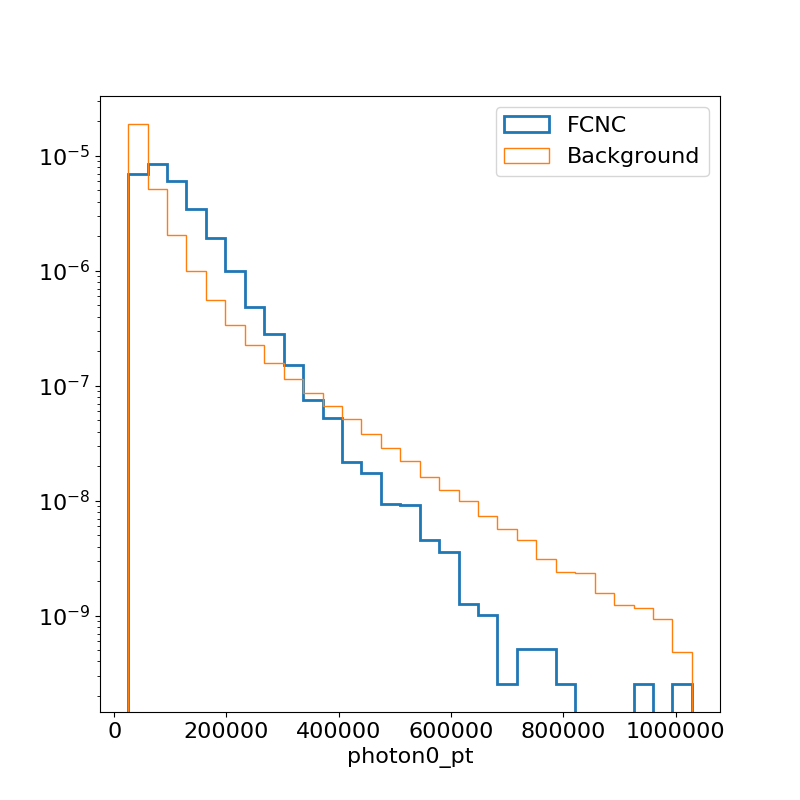
\includegraphics[width=.85\textwidth]{Images/ejetsvarplots/photon0_pt.png} \\
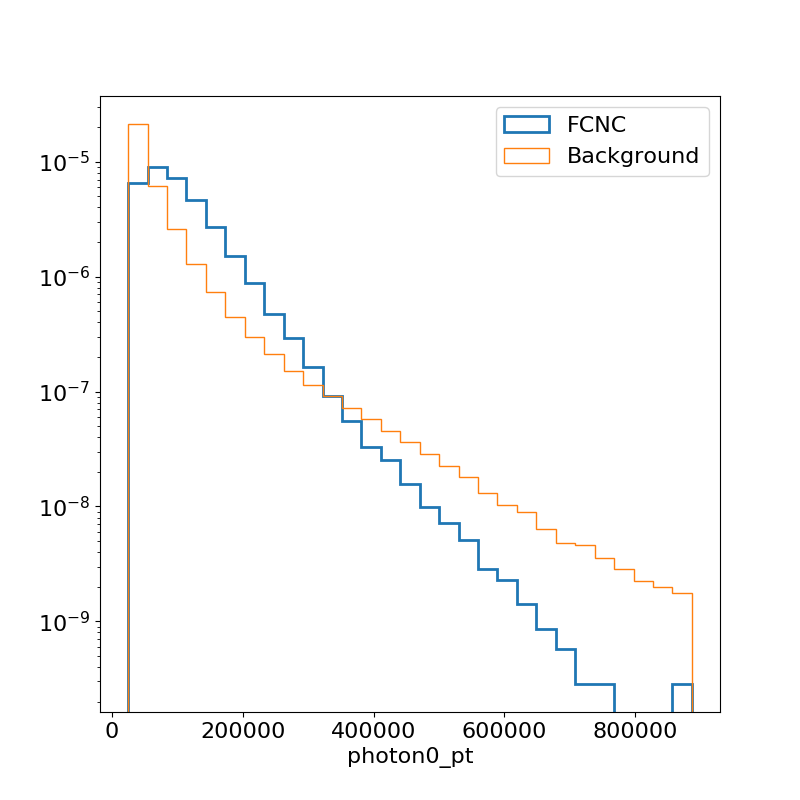
\includegraphics[width=.85\textwidth]{Images/mujetsvarplots/photon0_pt.png}
\end{column}
\begin{column}{0.33\textwidth}
\begin{itemize}
\item Lepton E
\end{itemize}
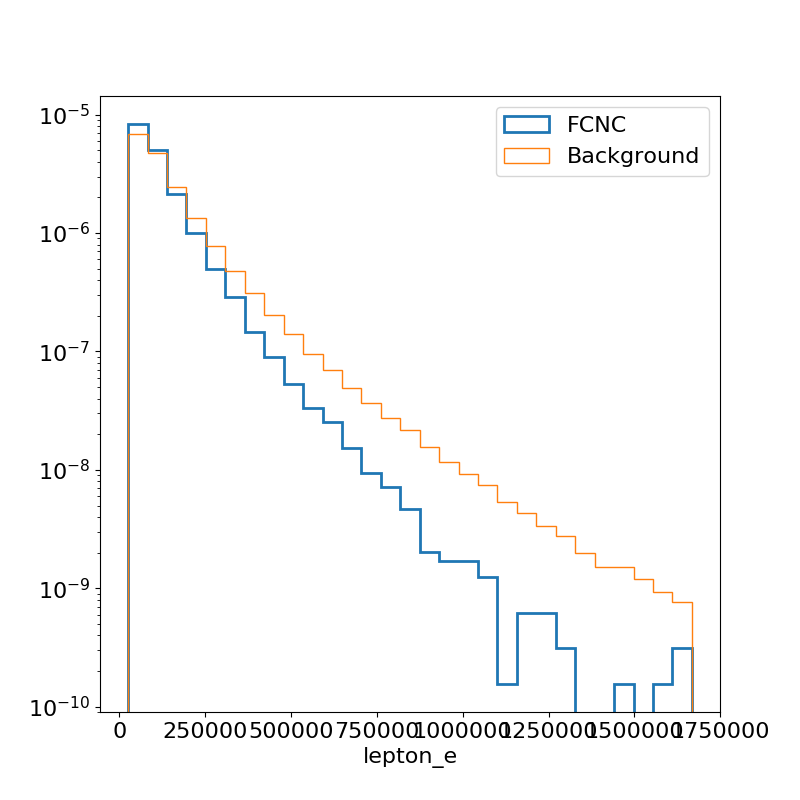
\includegraphics[width=.85\textwidth]{Images/ejetsvarplots/lepton_e.png} \\
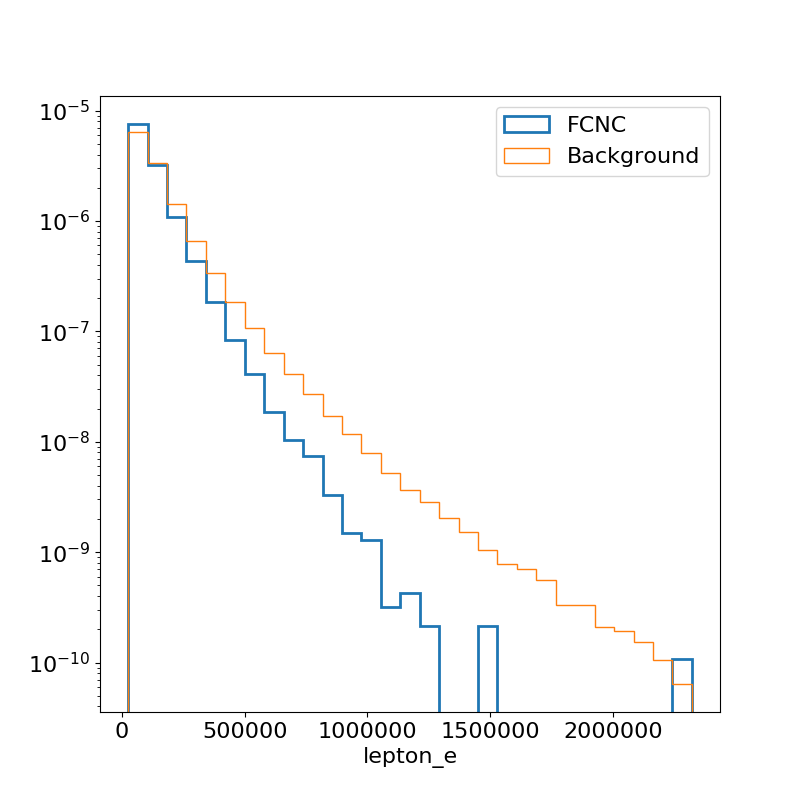
\includegraphics[width=.85\textwidth]{Images/mujetsvarplots/lepton_e.png}
\end{column}
\end{columns}
}

\frame{\frametitle{Preselection Objects with $N_{BJet}= 1$ }
\begin{columns}
\begin{column}{0.02\textwidth}
\rotatebox{90}{Muon Channel \qquad  Electron Channel} 
%\rotatebox{90}{Muon Channel        } 
\end{column}
\begin{column}{0.33\textwidth}
\begin{itemize}
\item $\gamma_{iso}$
\end{itemize}
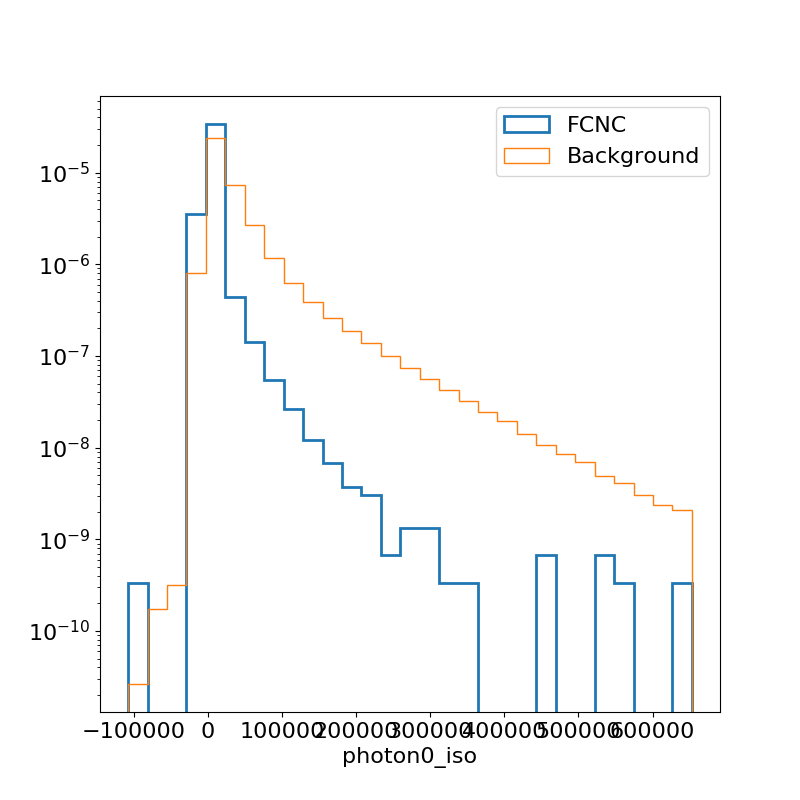
\includegraphics[width=.85\textwidth]{Images/ejetsvarplots/photon0_iso.png} \\
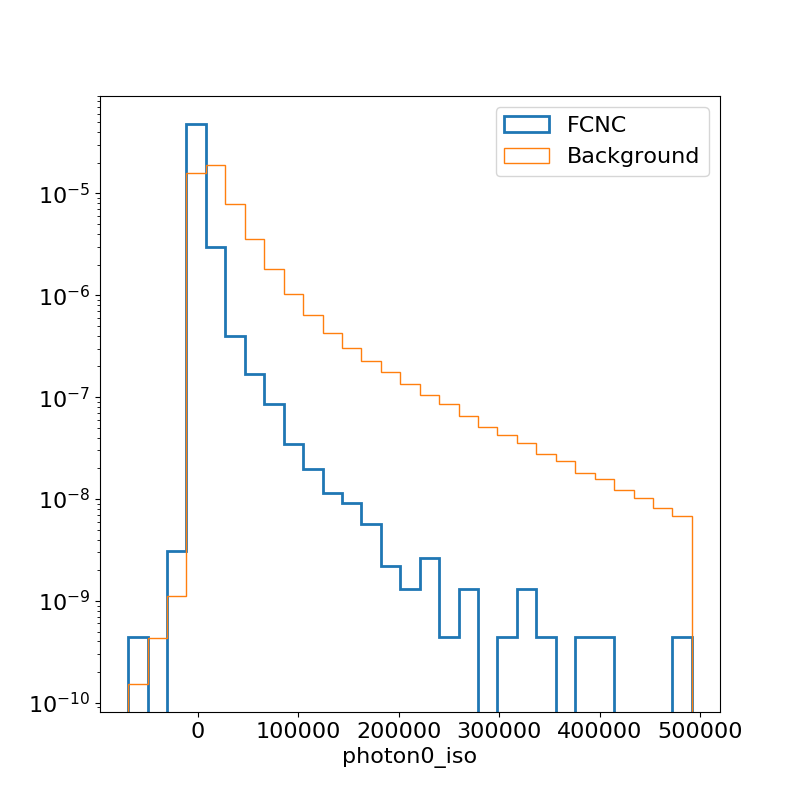
\includegraphics[width=.85\textwidth]{Images/mujetsvarplots/photon0_iso.png}
\end{column}
\begin{column}{0.33\textwidth}
\begin{itemize}
\item $\Delta R_{j\gamma}$
\end{itemize}
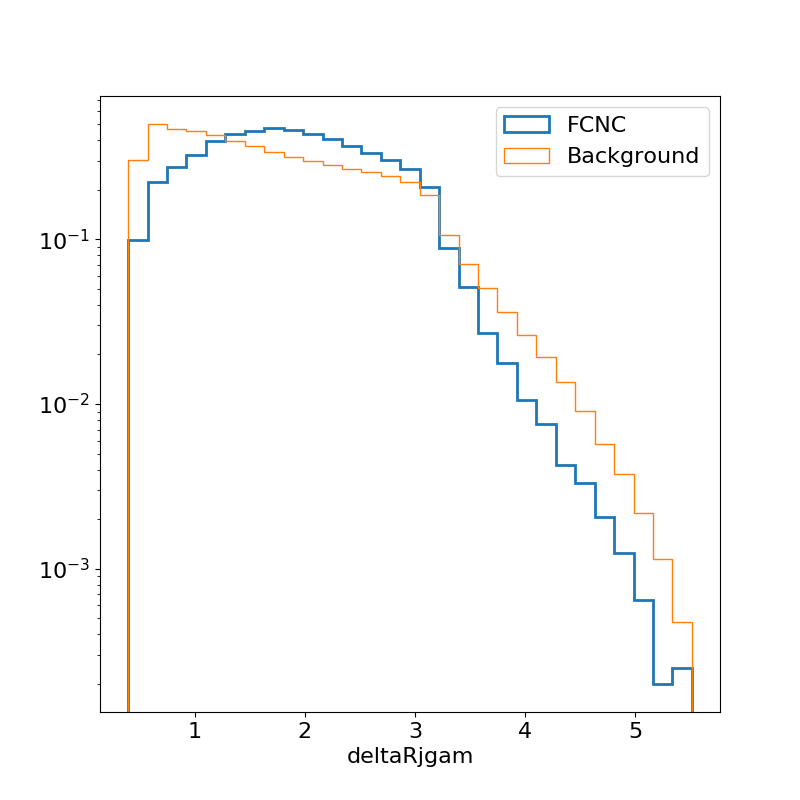
\includegraphics[width=.85\textwidth]{Images/ejetsvarplots/deltaRjgam.png} \\
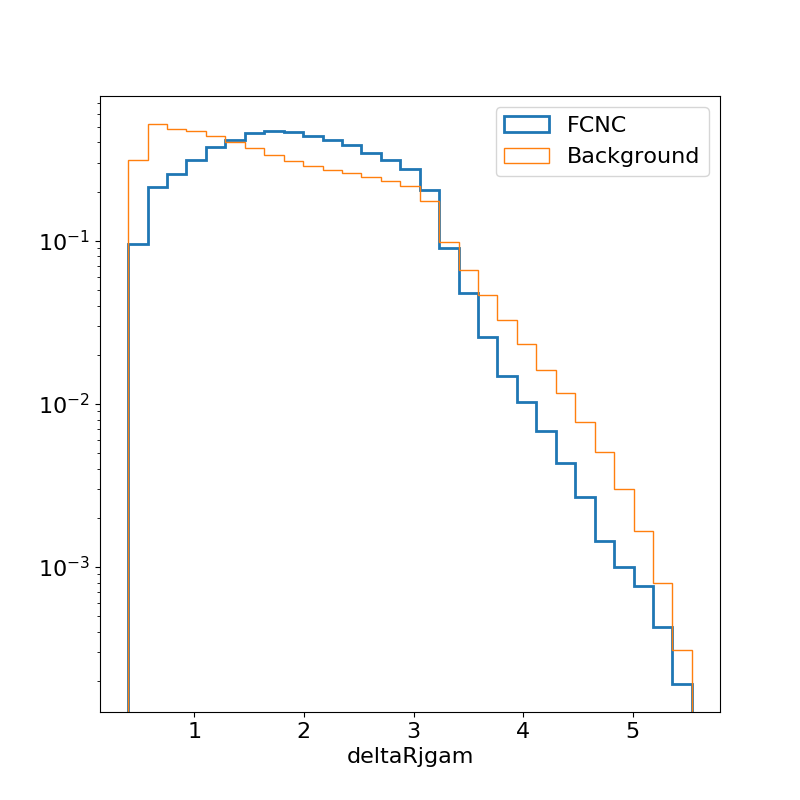
\includegraphics[width=.85\textwidth]{Images/mujetsvarplots/deltaRjgam.png}
\end{column}
\begin{column}{0.33\textwidth}
\begin{itemize}
\item $\Delta R_{l\gamma}$
\end{itemize}
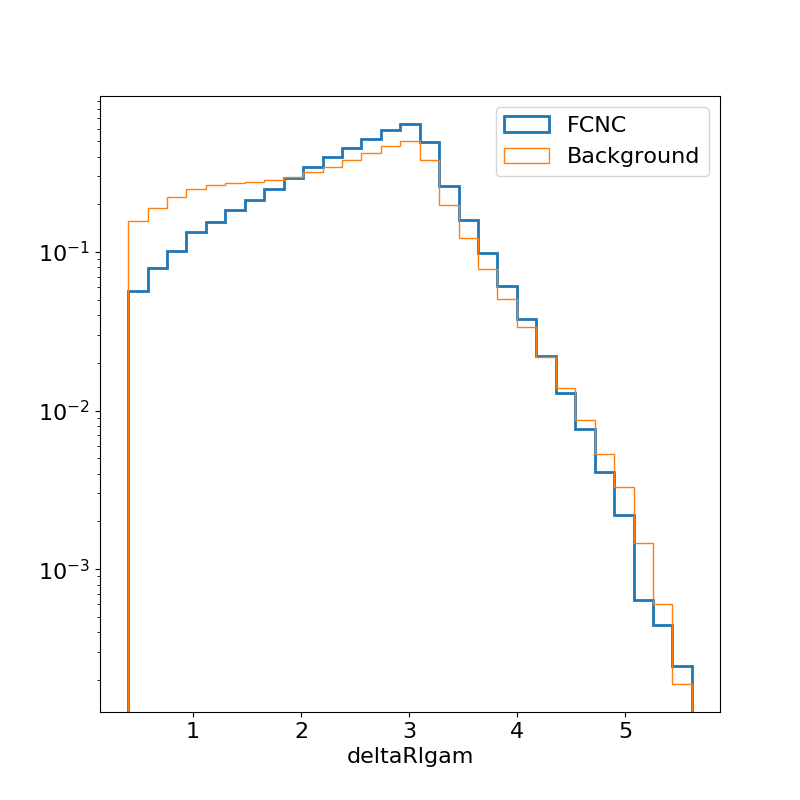
\includegraphics[width=.85\textwidth]{Images/ejetsvarplots/deltaRlgam.png} \\
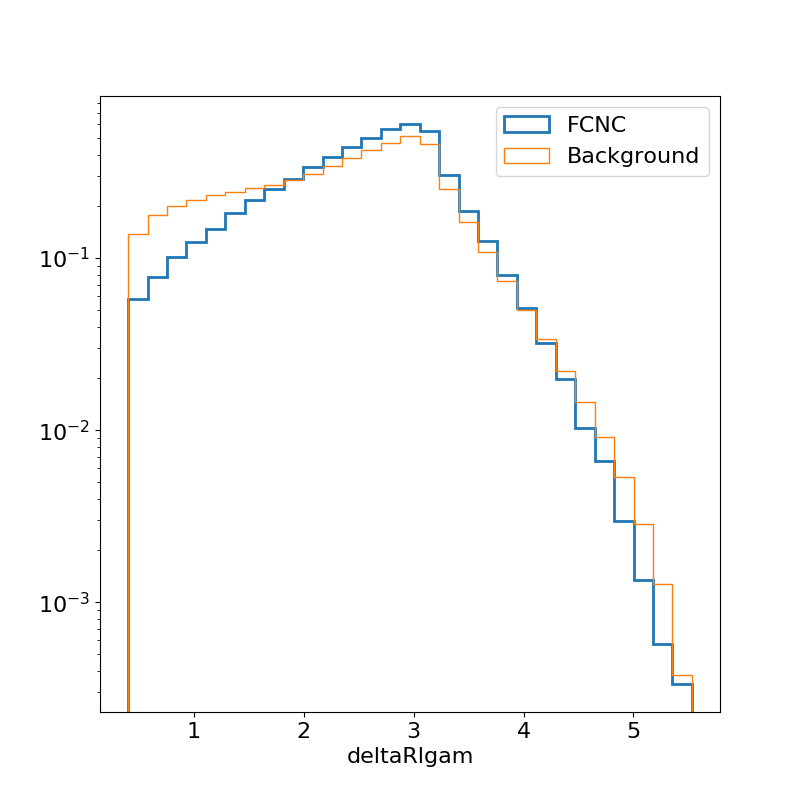
\includegraphics[width=.85\textwidth]{Images/mujetsvarplots/deltaRlgam.png}
\end{column}
\end{columns}
}

\subsection{Top and Neutrino Reconstruction}
\frame{\frametitle{Individual Top Reconstruction}
\begin{itemize}
\item  We can reconstruct top candidates from basic physics objects and $E_T^{miss}$
\item $E_T^{miss}$ is calculated to balance the event energy in the transverse plane of the detector
\item The other particles are combined in the only way the signal topology would allow two top quark candidates
\begin{itemize}
\item Standard model top candidate: b-jet + lepton + neutrino 
\item FCNC Top: Photon + Light Jet
\end{itemize}
\end{itemize}
}

%%%%%%%%%%%%%%%%


\frame{\frametitle{Neutrinos}
\begin{itemize}
\item All missing energy in signal topology is from neutrino
\item We have $E_T^{miss}$ and its direction   
\begin{itemize}
\item Can calulate  $E_{Tx}^{miss}$ and  $E_{Ty}^{miss}$ easily
\item Ambiguous direction along the z-axis
\end{itemize}
\item A minimization of this $\chi^2$ will allow us to determine the z momentum of the neutrino: $\chi^2 = \frac{(m_{b,l,\nu}-m_t)^2}{\sigma^2_{SMtop}}+\frac{(m_{l,\nu}-m_W)^2}{\sigma^2_W} $
\end{itemize}

%\[ \chi^2 = \frac{(m_{b,l,\nu}-m_t)^2}{\sigma^2_{SMtop}}+\frac{(m_{l,\nu}-m_W)^2}{\sigma^2_W}  \]
\begin{columns}
\begin{column}{0.5\textwidth}
\centering
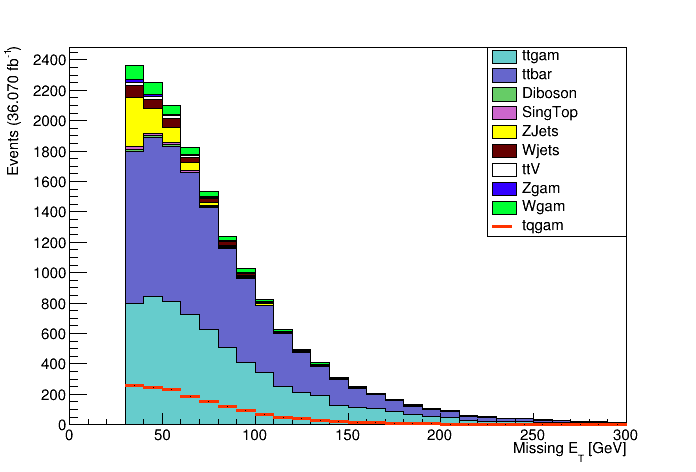
\includegraphics[width=.9\textwidth]{../../Thesis/ThesisImages/plotsloose/el_h_met_met.png}
\captionof{figure}{e-channel $E_T^{miss}$ distribution}
\end{column} 
\begin{column}{0.5\textwidth}
\centering
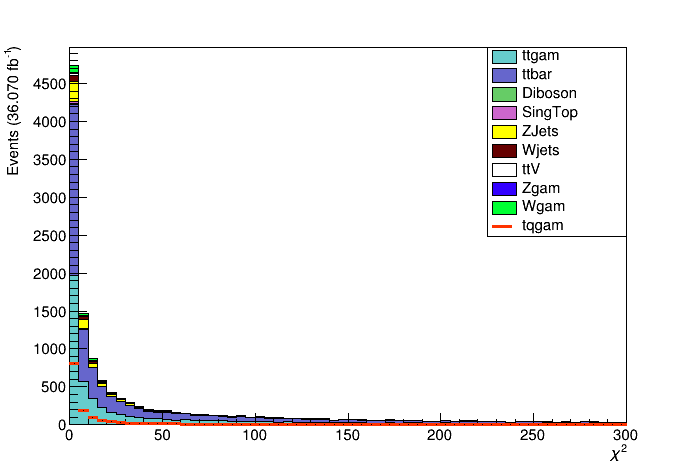
\includegraphics[width=.9\textwidth]{../../Thesis/ThesisImages/plotsloose/el_h_min_chi2.png}
\captionof{figure}{e-channel $\chi^2$ distribution}
\end{column}
\end{columns}
*Plots from previous release, same methodology used, same results
}

\frame{
\[ \chi^2 = \frac{(m_{b,l,\nu}-m_t)^2}{\sigma^2_{SMtop}}+\frac{(m_{l,\nu}-m_W)^2}{\sigma^2_W}  \]
\begin{columns}
\begin{column}{0.02\textwidth}
\rotatebox{90}{Muon Channel \qquad  Electron Channel} 
%\rotatebox{90}{Muon Channel        } 
\end{column}
\begin{column}{0.33\textwidth}
\begin{itemize}
\item $\chi^2$
\end{itemize}
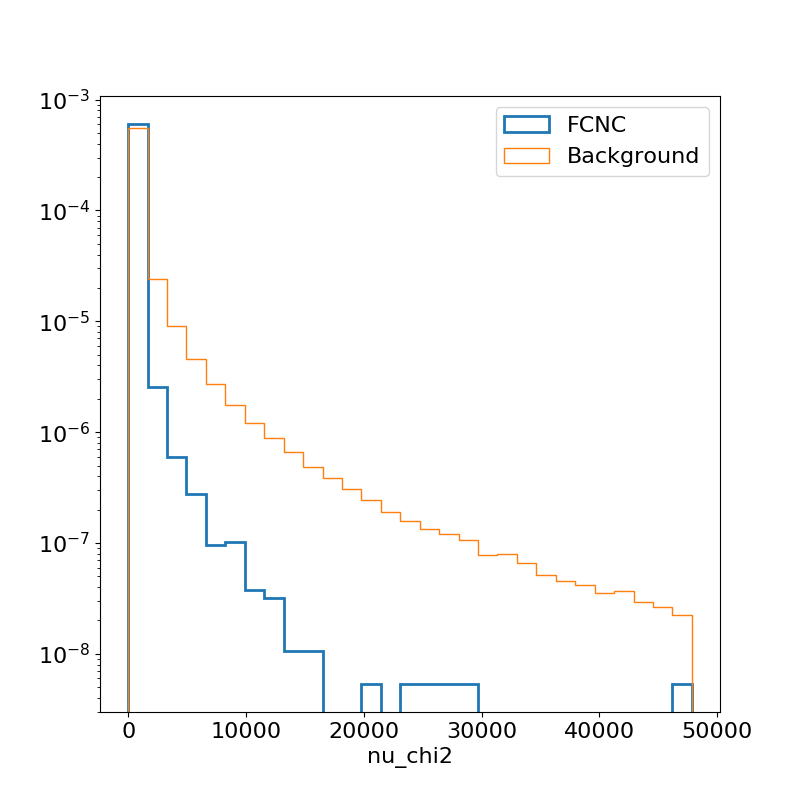
\includegraphics[width=.8\textwidth]{Images/ejetsvarplots/nu_chi2.png} \\
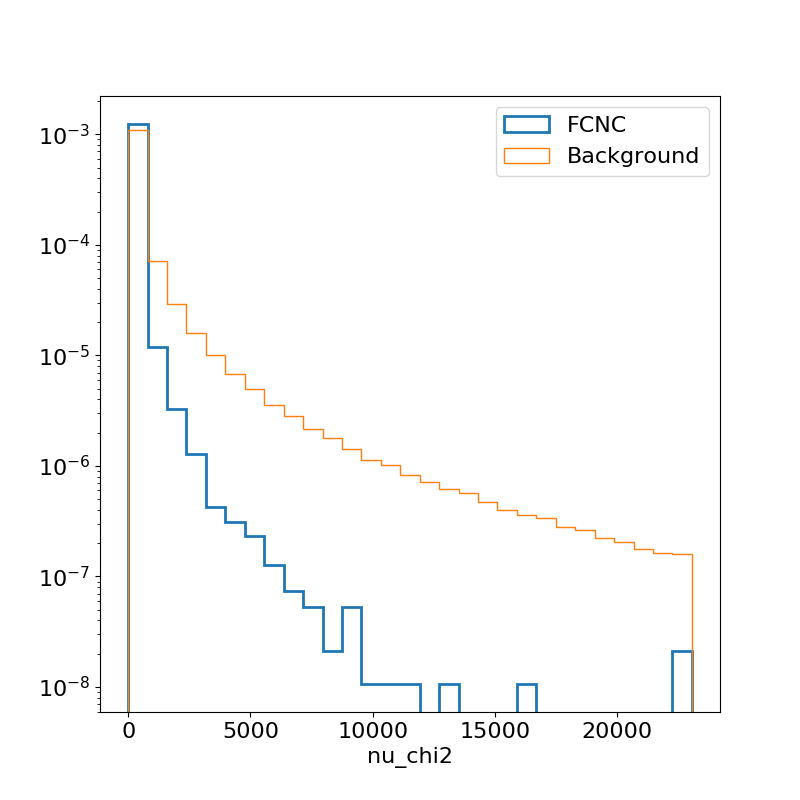
\includegraphics[width=.8\textwidth]{Images/mujetsvarplots/nu_chi2.png}
\end{column}
\begin{column}{0.33\textwidth}
\begin{itemize}
\item$\chi^2_{SMTop}$
\end{itemize}
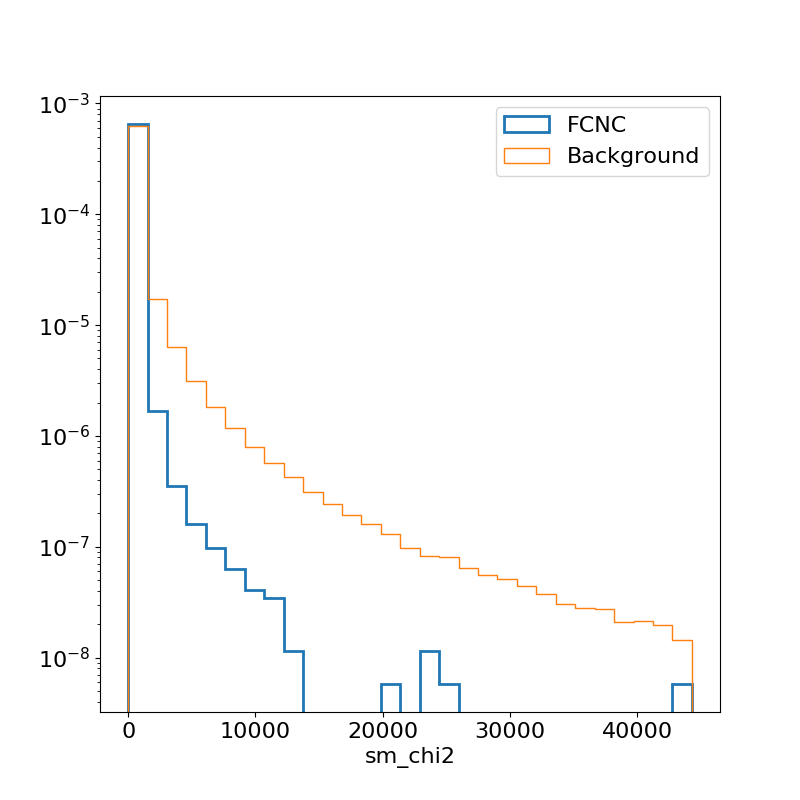
\includegraphics[width=.8\textwidth]{Images/ejetsvarplots/sm_chi2.png} \\
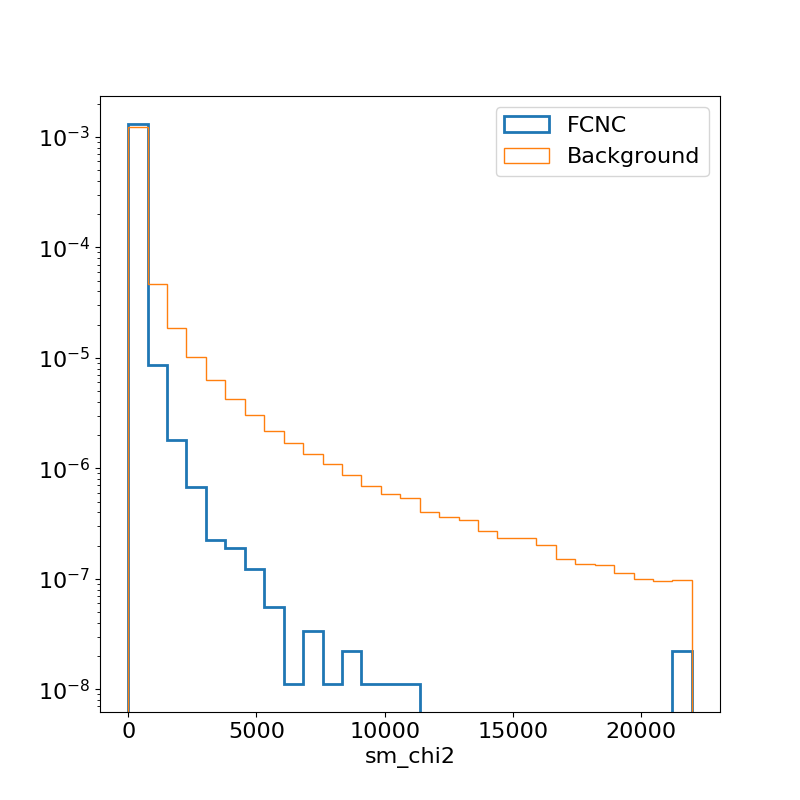
\includegraphics[width=.8\textwidth]{Images/mujetsvarplots/sm_chi2.png}
\end{column}
\begin{column}{0.33\textwidth}
\begin{itemize}
\item $\chi^2_{W}$
\end{itemize}
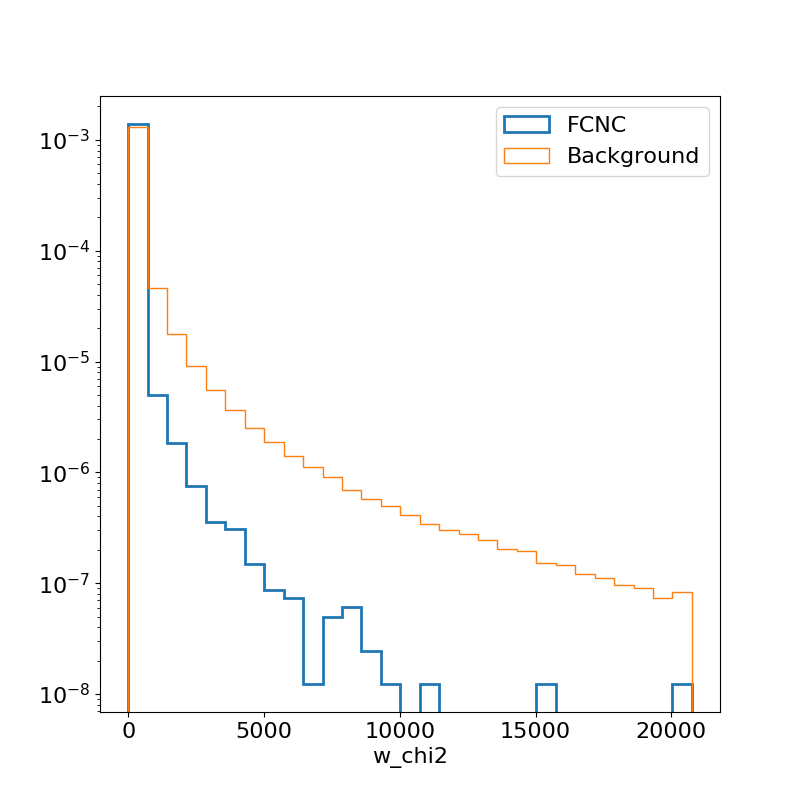
\includegraphics[width=.8\textwidth]{Images/ejetsvarplots/w_chi2.png} \\
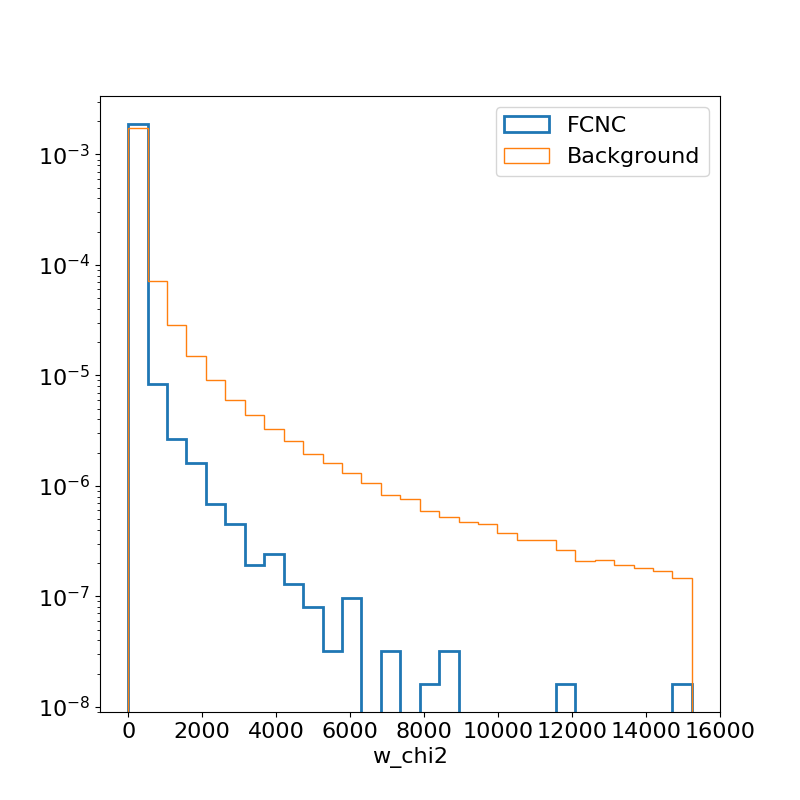
\includegraphics[width=.8\textwidth]{Images/mujetsvarplots/w_chi2.png}
\end{column}
\end{columns}
}

\section{Neural Network}
\subsection{Architecture}
\frame{\frametitle{Neural Network Architecture}
\begin{itemize}
\item Using Keras on top of Tensorflow various input parameters are tested for model behavior
\item A Dense Neural Network with variable number of input variables and hidden layers are explored
\item Cut optimization has been performed with full Run 2 luminosity for potential reach of the search
\end{itemize}
\centering
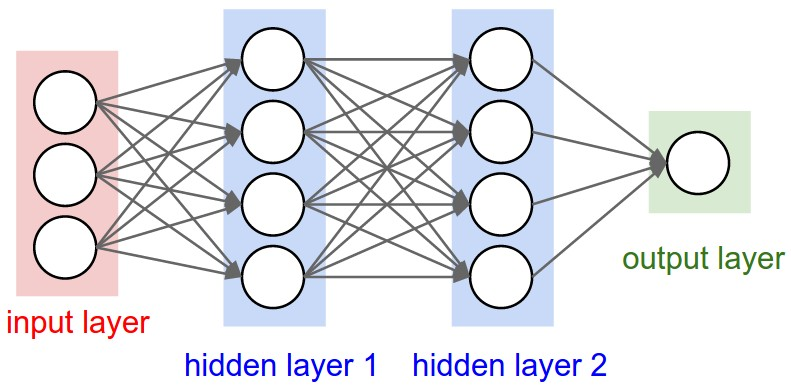
\includegraphics[width=0.7\textwidth]{Images/neural_net2.jpeg}
\captionof{figure}{\href{http://cs231n.github.io/neural-networks-1/}{[Ref: Neural Network]}}
}
\frame{\frametitle{Neural Network Optimizers}
\begin{itemize}
\item Various optimization functions can be used, however we use Adam (Adaptive Moment Estimation)
\begin{itemize}
\item Adam computes adaptive learning rates for every parameter and stores a history of the parameters used to calculate the next step
\item Stores first (mean) and second (uncentered variance) moments of the gradients used during training
\item Converges very fast and is less computationally intensive
\end{itemize}
\end{itemize}
\centering
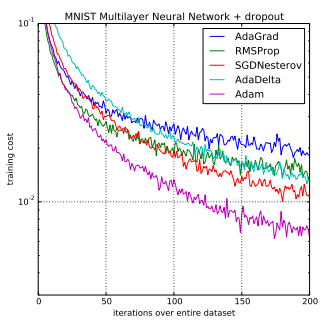
\includegraphics[width=0.35\textwidth]{Images/AdamComparison.png}
\captionof{figure}{\href{https://machinelearningmastery.com/adam-optimization-algorithm-for-deep-learning/}{[Ref:Machine Learning Mastry]}}
}

\frame{\frametitle{Neural Network Model Inputs}
\begin{itemize}
\item Using keras on top of tensorflow various input parameters are tested for model behavior
\item Networks are set up with 1 input layer, either 1 or 2 hidden layers with 10 nodes, and 1 output node
\item Each hidden layer has 20\% dropout to prevent overtraining by removing codependency between nodes
\item Batch size of 100 used and each network is allowed 200 epochs (with patience=50), all models converge and end early with reasonable batch sizes
\item Optimizer: Adam
\item Loss Function: Binary Cross Entropy
\end{itemize}
}

\frame{\frametitle{Neural Network Model Inputs}
\begin{itemize}
\item Minimal set of variables including kinematic and geometric variables chosen based on their separation power
\item Minimal variable set tested: $\gamma_{iso}$, $\gamma_{p_T}$,$\Delta R_{j\gamma}$,$\Delta R_{b l}$, $M_T^W$, $S_T$,$n_{jets}$,$\chi^2_W$, $\text{jet}_{0p_T}$,$\Delta R_{l\gamma}$,$\text{lepton}_E$, MET, $\text{bjet}_{0p_T}$
\item Add in extra variables to help training and see if improvement: High level variables/combinations that we know would be helpful in a cut based approach such as $m_{q\gamma}$,$m_{l\gamma}$, more $\chi^2$ fit information, etc.
\item A complex enough network should be able to figure out most of these straight forward combinations by itself 
\item Every MC sample is split into train/test/validation Sets (64\%,20\%,16\%) combined and shuffled for network analysis
\end{itemize}
}

\subsection{Neural Network Outcomes}
\frame{\frametitle{Neural Network, Electron Channel}
\begin{columns}
\begin{column}{0.48\textwidth}
\begin{itemize}
\item  Loss
\end{itemize}
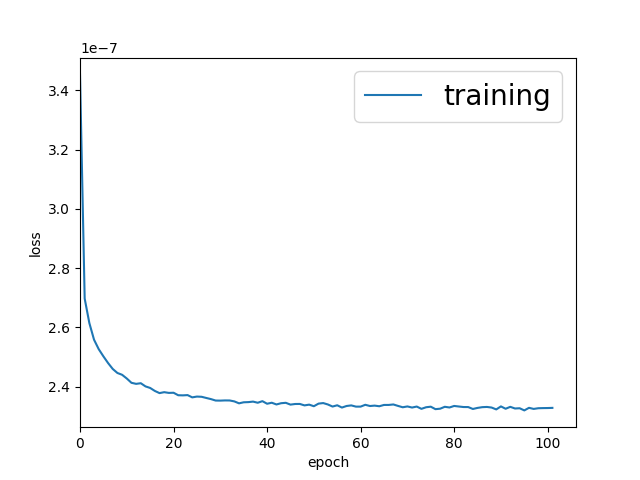
\includegraphics[width=.85\textwidth]{Images/ejetsOuts/loss.png}
\end{column}
\begin{column}{0.48\textwidth}
\begin{itemize}
\item Accuracy
\end{itemize}
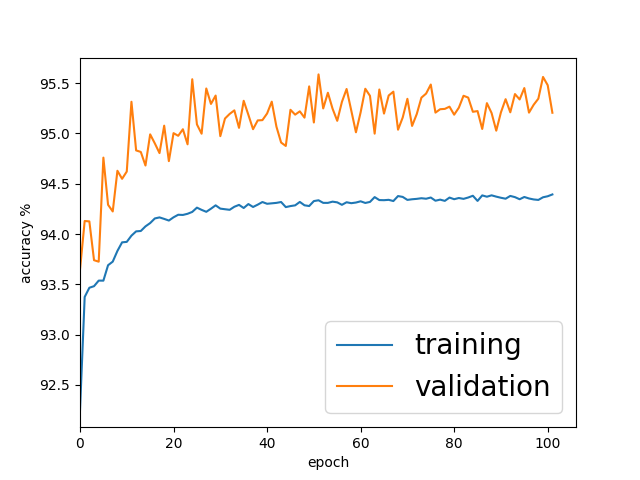
\includegraphics[width=.85\textwidth]{Images/ejetsOuts/accuarcy.png}
\end{column}
\end{columns}
}

\frame{\frametitle{Neural Network Separation, Electron Channel}
\begin{columns}
\begin{column}{0.02\textwidth}
\rotatebox{90}{Minimal Inputs \qquad \qquad Extended Inputs \qquad} 
%\rotatebox{90}{Muon Channel        } 
\end{column}
\begin{column}{0.48\textwidth}
\begin{itemize}
\item  1 Hidden Layer
\end{itemize}
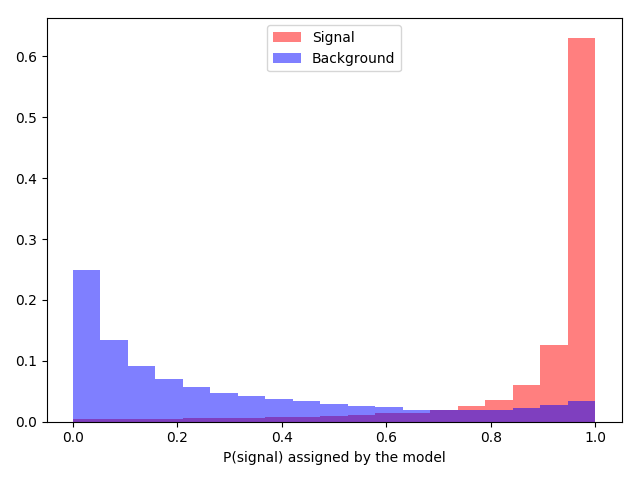
\includegraphics[width=.85\textwidth]{SmallNpart1modelouts/ejetsboth1hidnpart0sigbkg.png} \\
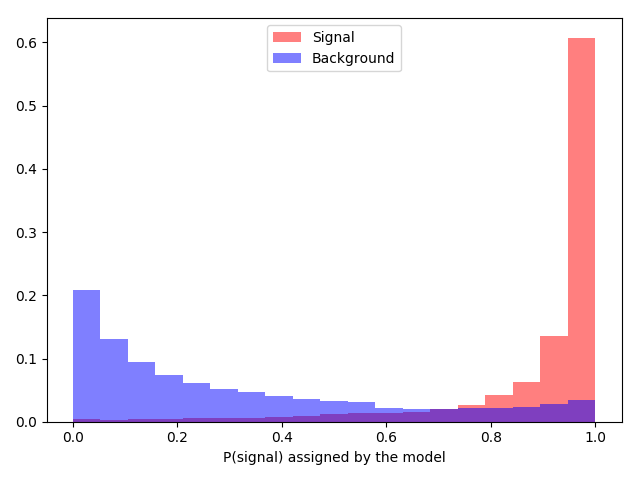
\includegraphics[width=.85\textwidth]{SmallNpart1modelouts/ejetsboth1hidnpart1sigbkg.png}
\end{column}
\begin{column}{0.48\textwidth}
\begin{itemize}
\item 2 Hidden Layers
\end{itemize}
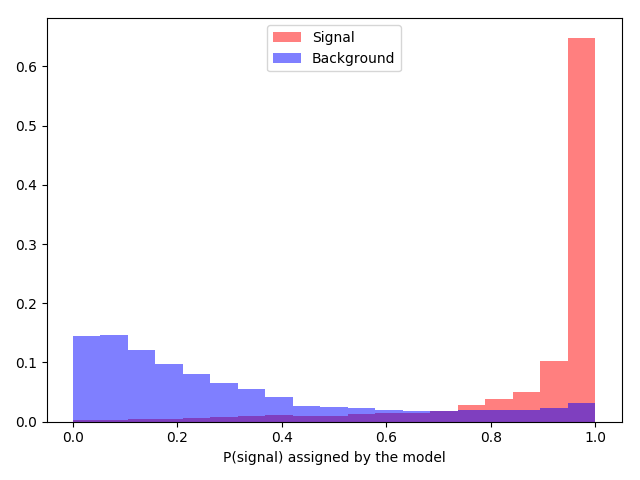
\includegraphics[width=.85\textwidth]{SmallNpart1modelouts/ejetsboth2hidnpart0sigbkg.png} \\
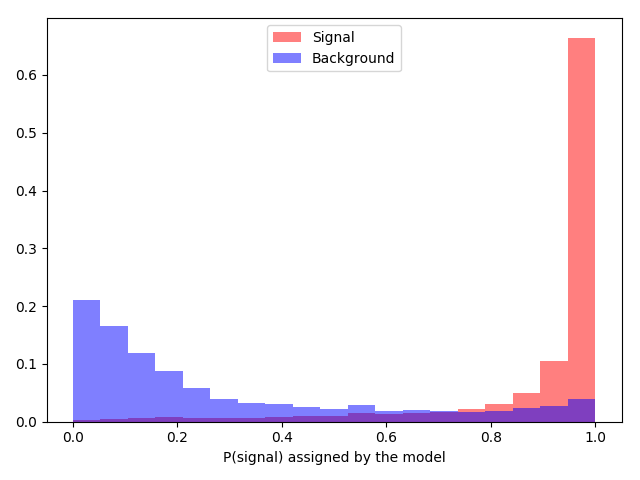
\includegraphics[width=.85\textwidth]{SmallNpart1modelouts/ejetsboth2hidnpart1sigbkg.png}
\end{column}
\end{columns}
}

\frame{\frametitle{Neural Network Separation, Muon Channel}
\begin{columns}
\begin{column}{0.02\textwidth}
\rotatebox{90}{Minimal Inputs \qquad \qquad Extended Inputs\qquad} 
%\rotatebox{90}{Muon Channel        } 
\end{column}
\begin{column}{0.48\textwidth}
\begin{itemize}
\item  1 Hidden Layer
\end{itemize}
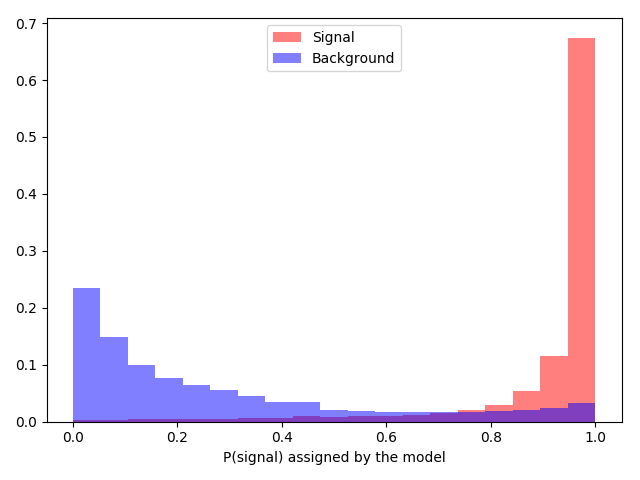
\includegraphics[width=.85\textwidth]{Images/modelouts/mujetsboth1hidnpart0sigbkg.png} \\
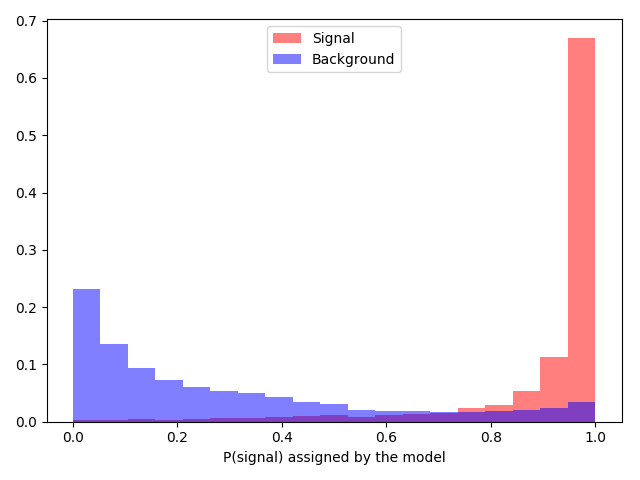
\includegraphics[width=.85\textwidth]{Images/modelouts/mujetsboth1hidnpart1sigbkg.png}
\end{column}
\begin{column}{0.48\textwidth}
\begin{itemize}
\item 2 Hidden Layers
\end{itemize}
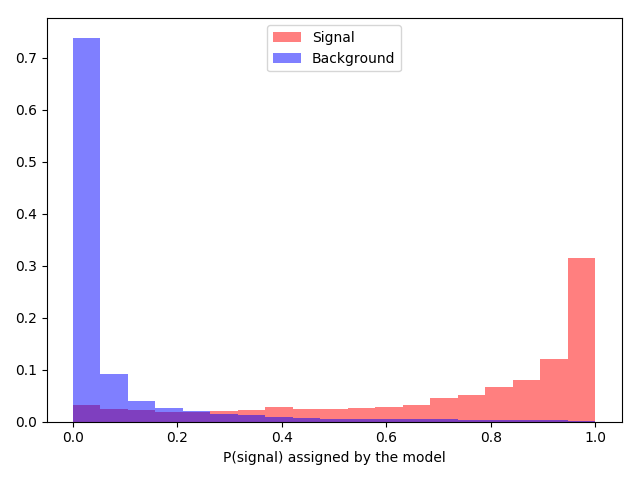
\includegraphics[width=.85\textwidth]{Images/modelouts/mujetsboth2hidnpart0sigbkg.png} \\
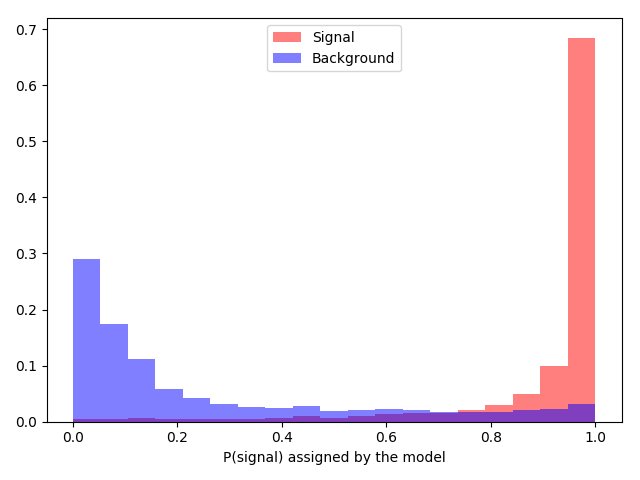
\includegraphics[width=.85\textwidth]{Images/modelouts/mujetsboth2hidnpart1sigbkg.png}
\end{column}
\end{columns}
}

\frame{\frametitle{ROC Curves for Multiple Models}
\begin{columns}
%\begin{column}{0.02\textwidth}
%\rotatebox{90}{Muon Channel \qquad  Electron Channel} 
%\rotatebox{90}{Muon Channel        } 
%\end{column}
\begin{column}{0.5\textwidth}
\begin{itemize}
\item Electron Channel
\end{itemize}
%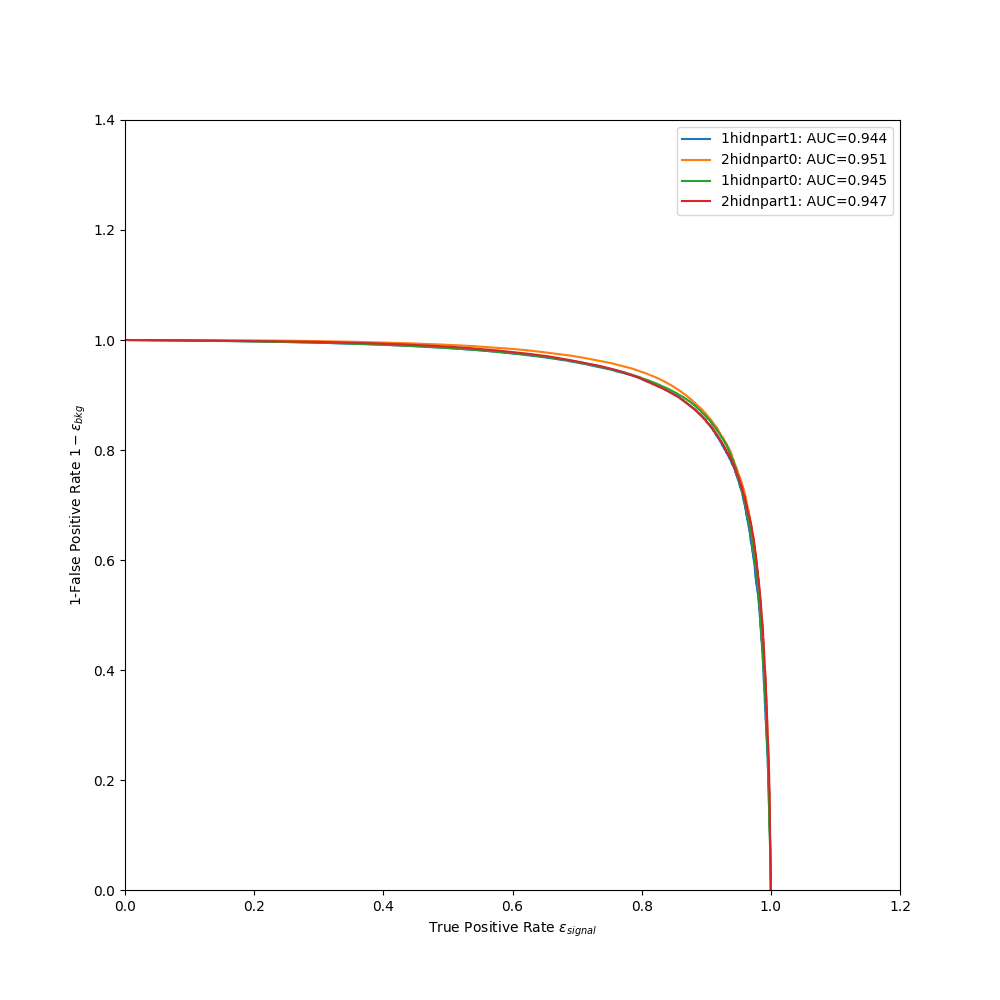
\includegraphics[width=1.0\textwidth]{Images/modelouts/ejetsbothroc.png} 
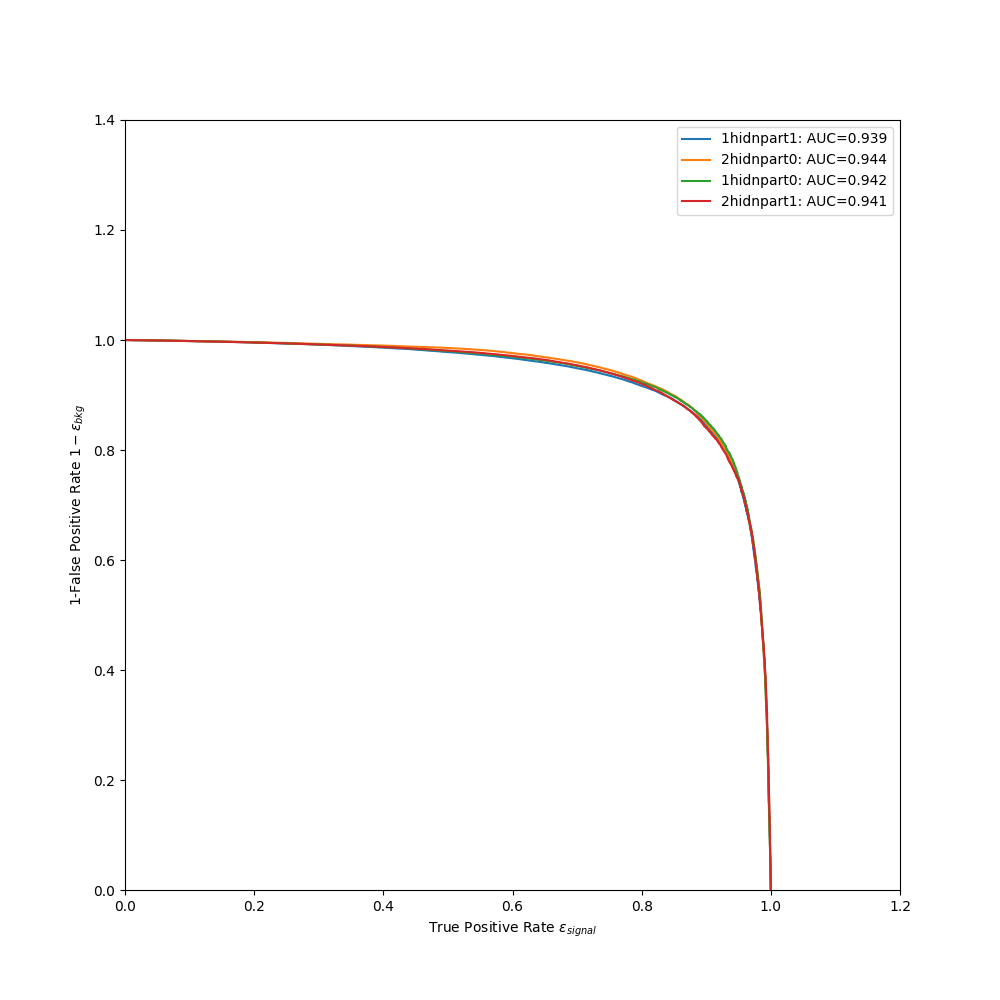
\includegraphics[width=1.0\textwidth]{SmallNpart1modelouts/ejetsbothroc.png} 
\end{column}
\begin{column}{0.5\textwidth}
\begin{itemize}
\item Muon Channel
\end{itemize}
\includegraphics[width=1.0\textwidth]{Images/modelouts/mujetsbothroc.png}
%\includegraphics[width=1.0\textwidth]{SmallNpart1modelouts/mujetsbothroc.png} 
\end{column}
\end{columns}
\begin{itemize}
\item All of these are very close (visually and by area), want to explore deeper to pick best model
\end{itemize}
}

\frame{\frametitle{Significance Plots, Electron Channel}
\begin{columns}
\begin{column}{0.02\textwidth}
\rotatebox{90}{Minimal Inputs \qquad Extended Inputs\qquad} 
%\rotatebox{90}{Muon Channel        } 
\end{column}
\begin{column}{0.48\textwidth}
\centering
\begin{itemize}
\item  1 Hidden Layer
\end{itemize}
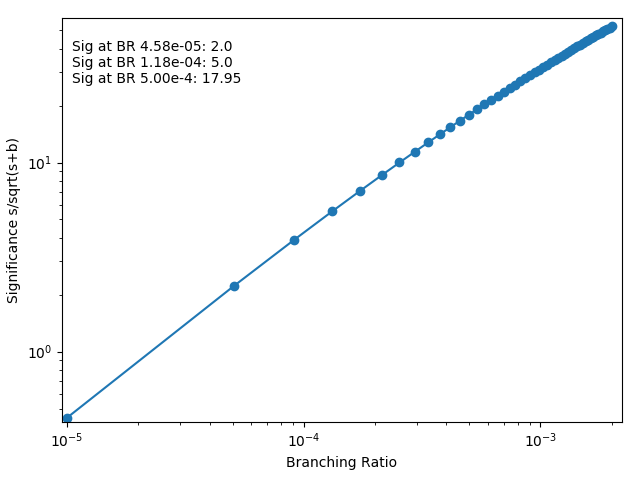
\includegraphics[width=0.7\textwidth]{SmallNpart1modelouts/ejetsboth1hidnpart0SigVsBR.png} 
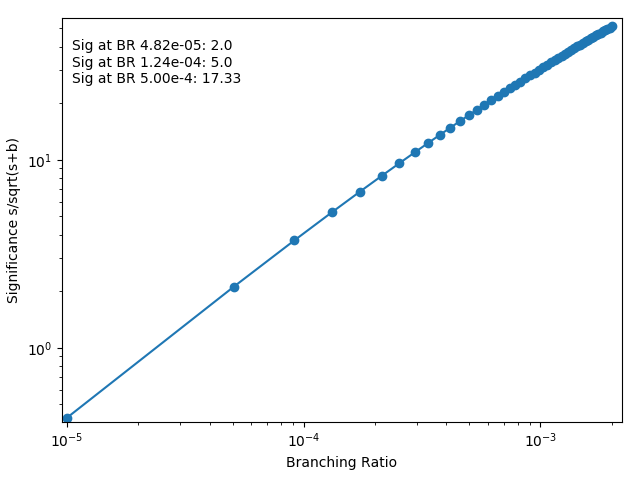
\includegraphics[width=0.7\textwidth]{SmallNpart1modelouts/ejetsboth1hidnpart1SigVsBR.png} 
\end{column}
\begin{column}{0.48\textwidth}
\centering
\begin{itemize}
\item 2 Hidden Layers
\end{itemize}
{%
\setlength{\fboxsep}{0pt}%
\setlength{\fboxrule}{1pt}%
\fbox{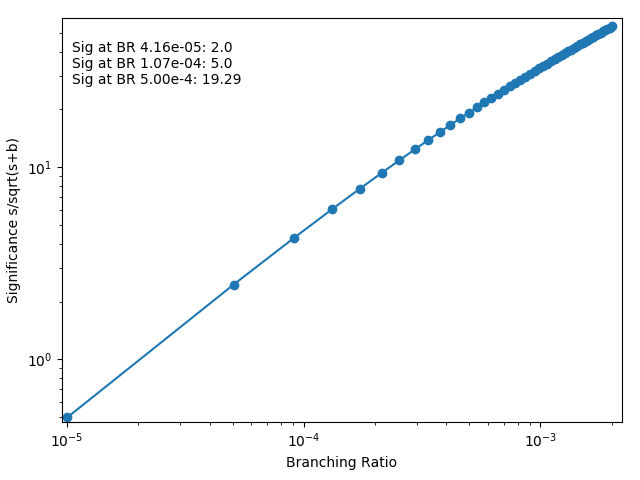
\includegraphics[width=0.7\textwidth]{SmallNpart1modelouts/ejetsboth2hidnpart0SigVsBR.png}}%
}\\
%\includegraphics[width=0.7\textwidth]{Images/modelouts/ejetsboth2hidnpart0SigVsBR.png} 
\includegraphics[width=0.7\textwidth]{SmallNpart1modelouts/ejetsboth2hidnpart1SigVsBR.png}
\end{column}
\end{columns}
\begin{itemize}
\item Significance:  S=$\frac{n_{S}}{\sqrt{n_{S}+n_{B}}}$
\end{itemize}
}

\frame{\frametitle{Significance Plots, Electron Channel}
\begin{columns}
\begin{column}{0.48\textwidth}
\centering
\includegraphics[width=0.85\textwidth]{Images/ejetsOuts/sigbkg.png} 
\includegraphics[width=0.85\textwidth]{Images/ejetsOuts/significance2.png} 
\end{column}
\begin{column}{0.48\textwidth}
\centering
\includegraphics[width=0.85\textwidth]{Images/ejetsOuts/SigVsBR.png} 
\includegraphics[width=0.85\textwidth]{Images/ejetsOuts/CutVsBR.png} 
\end{column}
\end{columns}
}
\frame{\frametitle{Significance Plots, Muon Channel}
\begin{columns}
\begin{column}{0.48\textwidth}
\centering
\includegraphics[width=0.85\textwidth]{Images/mujetsOuts/sigbkg.png} 
\includegraphics[width=0.85\textwidth]{Images/mujetsOuts/significance2.png} 
\end{column}
\begin{column}{0.48\textwidth}
\centering
\includegraphics[width=0.85\textwidth]{Images/mujetsOuts/SigVsBR.png} 
\includegraphics[width=0.85\textwidth]{Images/mujetsOuts/CutVsBR.png} 
\end{column}
\end{columns}
}

\frame{\frametitle{Cut Optimization}
\begin{itemize}
\item Cut optimization gives a pretty consistent value for a wide range of Branching Ratios
\item Close depending on the model but can differ slightly if optimizing for discovery vs. optimal limit setting 
\item To reasonable precision the suggested cuts from the previous plots are identical $\text{NN}_{\text{cut}}=0.98$ for both channels
\item Can implement this cut going forward with the rest of the analysis and make sure it behaves in various orthogonal control and validation regions
\end{itemize}
}


\section{Continuing Analysis}
\subsection{Region Creation}
\frame{\frametitle{Validation Region - With Real Photons}
\begin{itemize}
\item Validation and Control Regions are created orthogonal to Signal Region for large backgrounds
\item VR for ($t\bar{t}+\gamma$)
\begin{itemize}
\item Same preselection cuts as SR
\item $>4$ jets
\item Reverse FCNC top mass cut $|m_{q\gamma}-m_{top}|>50GeV$: Guarantees orthogonality 
\end{itemize}
\item VR for $W+\gamma$
\begin{itemize}
\item Similar preselection cuts to SR
\item = 0 BJets (orthogonal cut)
\end{itemize}
\item Similar regions have been created for regions without real photons - included in recent grid run
\begin{itemize}
\item These regions include $t\bar{t}$ and $W$ rich samples with 0 good photons and different amounts of jets
\item Including these regions greatly increases processing time necessary because of glut of 0b/0$\gamma$ events - Requires reoptimization of current analysis code
\end{itemize}
\end{itemize}
}


%%%%%%%%%%%%%%%%%%%%%%%%%%%%%%%%%%%%%%%%%%%%%%%%%%%%%%%%%%%%%%%%%%
\section{Outlook and Conclusions}

\frame{\frametitle{Outlook}
\begin{itemize}
\item Still lots to be done
\item Fake Rates $e\rightarrow\gamma$ and $j\rightarrow\gamma$ will be investigated next
\item Full MC grid run of MC16a/d/e samples is complete, using for current investigations
\item Full Analysis transitioned to be able to run on condor nodes
\begin{itemize}
\item  Capable of handling much larger samples by directly using grid output files
\item Necessary to look at MC16a/d/e samples and full 2018 data set in a reasonable amount of time (especially with VRs/CRs)
\end{itemize}
\item Initial neural network studies are completing, can push forward with another step of the analysis
\end{itemize}
}



\frame{\frametitle{Conclusion}
\begin{itemize}
\item Any excess signal would be indicative of some physics beyond the Standard Model that couples strongly to the top sector
\item With the inclusion of the neural network significant gains can be made in the search for FCNCs with top quark decays 
\item FCNCs with enhanced rates are important pieces for testing many new theories
\item Analysis is going after a long lull due to MC Production delays
\item Thank you!
\end{itemize}
}


%%%%%%%%%%%%%%%%%%%%%%%%%%%%%%%%%%%%%%%%%%%%%%%%%%%%%%%%%%%%%%%%

\appendix
\section{Backup}
\frame{\frametitle{Backup}
}
\frame{\frametitle{NN Input Variable Correlations}
\centering
\includegraphics[height=.8\textheight]{Images/correlations.png}
}

\frame{\frametitle{Neural Network Model Inputs}
\centering
\scalebox{0.8}{ $\text{Separation} = \sum_{i}^{bins} \frac {n_{s i}-n_{b i}}{n_{s i}+n_{b i}}$}
\begin{columns}
\begin{column}{0.48\textwidth}
\centering
mu+jets channel\\
\scalebox{0.6}{\begin{tabular}{cc}
Variable & Separation \\
\hline
photon0iso & 41.18 \\
mqgam & 28.27 \\
photon0pt & 24.07 \\
mtSM & 11.60 \\
mlgam & 7.56 \\
deltaRjgam & 5.64 \\
deltaRbl & 4.42 \\
MWT & 3.34 \\
ST & 3.30 \\
nuchi2 & 3.12 \\
jet0pt & 2.81 \\
njets & 2.07 \\
smchi2 & 1.89 \\
wchi2 & 1.87 \\
jet0e & 1.52 \\
deltaRlgam & 1.17 \\
leptone & 0.87 \\
deltaRjb & 0.86 \\
met & 0.68 \\
bjet0pt & 0.52 \\
leptoniso & 0.27 \\
\end{tabular}
}
\end{column}
\begin{column}{0.48\textwidth}
\centering
e+jets channel \\
\scalebox{0.6}{\begin{tabular}{c c}
Variable & Separation\\
\hline
photon0pt & 23.14 \\
mqgam & 22.73 \\
photon0iso & 18.70 \\
mtSM & 11.02 \\
mlgam & 9.53 \\
deltaRbl & 5.00 \\
deltaRjgam & 4.60 \\
ST & 3.83 \\
MWT & 3.16 \\
jet0pt & 2.47 \\
njets & 1.70 \\
nuchi2 & 1.59 \\
deltaRlgam & 1.40 \\
wchi2 & 1.33 \\
smchi2 & 1.09 \\
deltaRjb & 0.88 \\
leptone & 0.85 \\
leptoniso & 0.56 \\
bjet0pt & 0.50 \\
met & 0.47 \\
\end{tabular}
}
\end{column}
\end{columns}
}

\frame{\frametitle{Input Variables}
Extended Inputs: [`photon0iso','photon0pt','mqgam','mlgam','mtSM', 'deltaRjgam','deltaRbl','MWT','ST','njets','nbjets','wchi2','jet0pt', 'deltaRlgam', 'leptone','met','bjet0pt']
\\ 
Minimal Inputs: ['photon0iso','photon0pt','deltaRjgam','deltaRbl','MWT', 'ST','njets','wchi2','jet0pt','deltaRlgam','leptone','met','bjet0pt']
}

\frame{\frametitle{Integrated Luminosity}
\centering
\includegraphics[width=1.\textwidth]{../../Thesis/ThesisImages/2017PeakLumiByFill.pdf}
}
\frame{\frametitle{A Couple BSM Diagrams}
\centering
\includegraphics[width=1.\textwidth]{../../Thesis/ThesisImages/BSMDiagrams.png}
}

\frame{\frametitle{Jets/AntiKT}

\[ d_{ij} = min(\frac{1}{p_{ti}^2},\frac{1}{p_{tj}^2}) \frac{\Delta_{ij}^2}{R^2}
\]
\[ d_{iB} = \frac{1}{p_{ti}^2}
\]
\[ \Delta_{ij}^2 = (\eta_i -\eta_j )^2 + (\phi_i - \phi_j )^2
\]
\begin{itemize}
\item Find minimum of entire set of $\{ d_{ij},d_{iB} \}$
\item If $d_{ij}$ is the minimum particles i,j are combined into one particle and removed from the list of particles
\item If $d_{iB}$ is the minimum i is labelled as a final jet and removed from the list of particles
\item Repeat until all particles are part of a jet with distance between jet axes $\Delta_{ij}$ is greater than R
\end{itemize}
}

\frame{\frametitle{B-tagging}
\centering
\includegraphics[height=.8\textheight]{../../Thesis/ThesisImages/B-tagging_diagram.png}
}

\frame{\frametitle{}
\[ \mathcal{L}^{eff}_{tq\gamma} = - e \bar{c} \frac{i \sigma^{\mu\nu}q_{\nu}}{m_t}(\lambda^{L}_{ct}P_L + \lambda^{R}_{ct}P_{R}) t A_{\mu} +H.c.
\]
}

\end{document}

%36.070


%%% Neural Net Ref: http://cs231n.github.io/neural-networks-1/

% npart0=['photon0_iso','photon0_pt','m_qgam','m_lgam','m_tSM','deltaRjgam','deltaRbl','MWT','S_T','nbjets','njets','w_chi2','jet0_pt','nu_chi2','sm_chi2','deltaRlgam','lepton_e','met','lepton_iso','bjet0_pt']
%all vars

%npart = ['photon0_iso','photon0_pt','m_qgam','m_lgam','m_tSM','deltaRjgam','deltaRbl','MWT','S_T','njets','nbjets','w_chi2','jet0_pt','deltaRlgam','lepton_e','met','bjet0_pt']
%usual npart1

%npart1=['photon0_iso','photon0_pt','deltaRjgam','deltaRbl','MWT','S_T','njets','w_chi2','jet0_pt','deltaRlgam','lepton_e','met','bjet0_pt']
%minimal